\documentclass[conference]{IEEEtran}
\IEEEoverridecommandlockouts
% The preceding line is only needed to identify funding in the first footnote. If that is unneeded, please comment it out.

%\usepackage[utf8]{inputenc}
%\usepackage{cite}
\usepackage{amsmath,amssymb,amsfonts}
\usepackage{algorithmic}
\usepackage[tight,footnotesize]{subfigure}
\usepackage{graphicx}
\usepackage{textcomp}
\usepackage{xcolor}
\usepackage[noadjust]{cite} %[5]-[12]
%\usepackage[ruled,vlined]{algorithm2e}
\usepackage{balance} 

%\linespread{0.992}

\begin{document}

\bstctlcite{IEEEexample:BSTcontrol}
\title{Future Generation Multi-tier Video Streaming Networks}

\author{\IEEEauthorblockN{1\textsuperscript{st} Given Name Surname}
\IEEEauthorblockA{\textit{dept. name of organization (of Aff.)} \\
\textit{name of organization (of Aff.)}\\
City, Country \\
email address}
\and
\IEEEauthorblockN{2\textsuperscript{nd} Given Name Surname}
\IEEEauthorblockA{\textit{dept. name of organization (of Aff.)} \\
\textit{name of organization (of Aff.)}\\
City, Country \\
email address}
\and
\IEEEauthorblockN{3\textsuperscript{rd} Given Name Surname}
\IEEEauthorblockA{\textit{dept. name of organization (of Aff.)} \\
\textit{name of organization (of Aff.)}\\
City, Country \\
email address}
}

\maketitle

\begin{abstract}
Video streaming services have been experiencing changes in the recent years, where the number of users consuming a variety of video streaming has been increasing exponentially in Video-on-Demand~(VoD) platforms. In order to accommodate the growing video traffic demand, new solutions have to be designed for the Future of the Internet to provide good users' Quality of Experience~(QoE).
However, a centralized cloud service has some problems, such as increased latency and congestion at the core of the network. Therefore, in order to improve video services, it is of utmost importance to properly distribute video streams according to your requirements: a real-time video infrastructure in a cloud is an interactive service that needs reduced delays (a few milliseconds), while a non-interactive VoD delivery can tolerate longer delays without impairing the quality of the experience. Proper management and orchestration of video delivery over the Internet is essential for the smooth coexistence of heterogeneous video services. This project proposes the use of the fog/cloud hierarchy to design a cooperative video streaming, implementing a set of mechanisms capable of offering an improved Quality of Experience~(QoE) to end users. In this way, this research project proposes to evaluate the impact on the performance of VoD introduced by new distributed computing infrastructures in edge/cloud computing scenarios.
%No entanto, um serviço de nuvem centralizado apresenta alguns problemas, como maior latência e congestionamento da núcleo da rede. Portanto, para melhorar os serviços de vı́deo, é de suma importância distribuir adequadamente os fluxos de vı́deo de acordo com seus requisitos: uma infraestrutura de vı́deos em tempo real em nu- vem é um serviço interativo que precisa de atrasos reduzidos (alguns milissegundos), enquanto uma entrega de VoD não interativa pode tolerar maior atraso sem prejudicar a qualidade da experiência. Um gerenciamento e orquestração adequados da entrega de video pela Internet é essencial para a coexistência suave de serviços de vı́deo heterogêneos. Este projeto propõe o uso da hierarquia de névoa/nuvem para projetar um streaming de video DASH cooperativo em Cidades Inteligentes, implantando um conjunto de mecanismos capaz de oferecer uma Qualidade de Experiência (QoE) aprimorada para usuários finais.
\end{abstract}

\begin{IEEEkeywords}
Edge computing, Cloud computing, Quality of Experience, Video Streaming, Video-on-Demand
\end{IEEEkeywords}


\section{Introduction}
\label{sec:introduction}

%{\color{blue} In this section we will contextualize video streaming technology and hierarchical caching problems, emphasizing the need of create a hierarchical topology to , and describe the content of each section of the paper.}

% Introduction of the Content and MEC service provider  
Over the years, Internet traffic has grown exponentially around the world. Mainly due to the multimedia content streaming, which, currently, represents 70\% of the whole traffic~\cite{cisco:forecast}. 
The Over-the-top~(OTT) provider can use the network edge to caching and transmit the video traffic with an uninterrupted streaming experience, at least as smooth as possible, to accommodate this growing video demand. This includes current video services as well as innovative services such as Real-time video streams and future games console~(e.g. AWS Wavelength and Google Stadia).
This trend imposes new challenges in video provisioning to satisfy the Quality of Experience~(QoE) guarantees for a wide range of users subscribers. As it is originally designed to consider the best-effort internet model for data transmission~\cite{gamaUCC2019, DBLP:CoRR:2021, ye:ITC17}.
%In order to provide the best user satisfaction, the advantages of high datarate and low latency in the edge network take into account today~\cite{gamaUCC2019, DBLP:CoRR:2021, ye:ITC17}. This trend imposes new challenges in providing videos with the best QoE, originally designed considering the best-effort internet model for data transmission.

In the moment that the content provider saturates available bandwidth or a particular set of service metrics across the network, the cloud server~(OTT provider) can reroute active connections to one or more edge caches that attend to the demand required. Such model can be represented by network organized hierarchically in multi-tiers to maintain a low traffic load~\cite{rosarioSENSORS2018}.
%When the content provider saturates the available bandwidth or a certain set of service metrics, the request may be routed to one or more edge caches. This model may be organized hierarchically in multi-tiers maintains a low traffic load~\cite{rosarioSENSORS2018}.

% Challenges
As well as the advantages of using the edge of the network with cache capabilities help user satisfaction, but it could bring negative impacts as well. When many users start to request video segments at the edge nodes, these surrogated nodes consider static users and just one edge node tiers. These nodes are not ready to deal with the constant changes in the number of users and the process of switching between different Access Points~(AP) due to user mobility.
Several works in the literature highlight edge/cloud computing to deal with the new video traffic demands, but there are aspects little addressed in user dynamic solutions. Figure~\ref{fig:multi-tier-network} depicts a multi-tier network architecture, which is composed of a heterogeneous set of devices and applications using distributed computing resources through multi-access communication technology, such as 5G and WiFi.
%
%Furthermore, the number of users connected in different APs changes accordingly to the surrogated edge nodes. For instance, a core network regional edge node provides video streaming to more users than an edge gateway. As shown in Fig.~\ref{fig:multi-tier-network}.
%
%Since the triggered video segments caching (replication) in an edge node.
%However, certain precautions when choosing the nodes for caching the video need to be taken into account. 

%Which it could result some issues. 

\begin{figure}
    \centering
    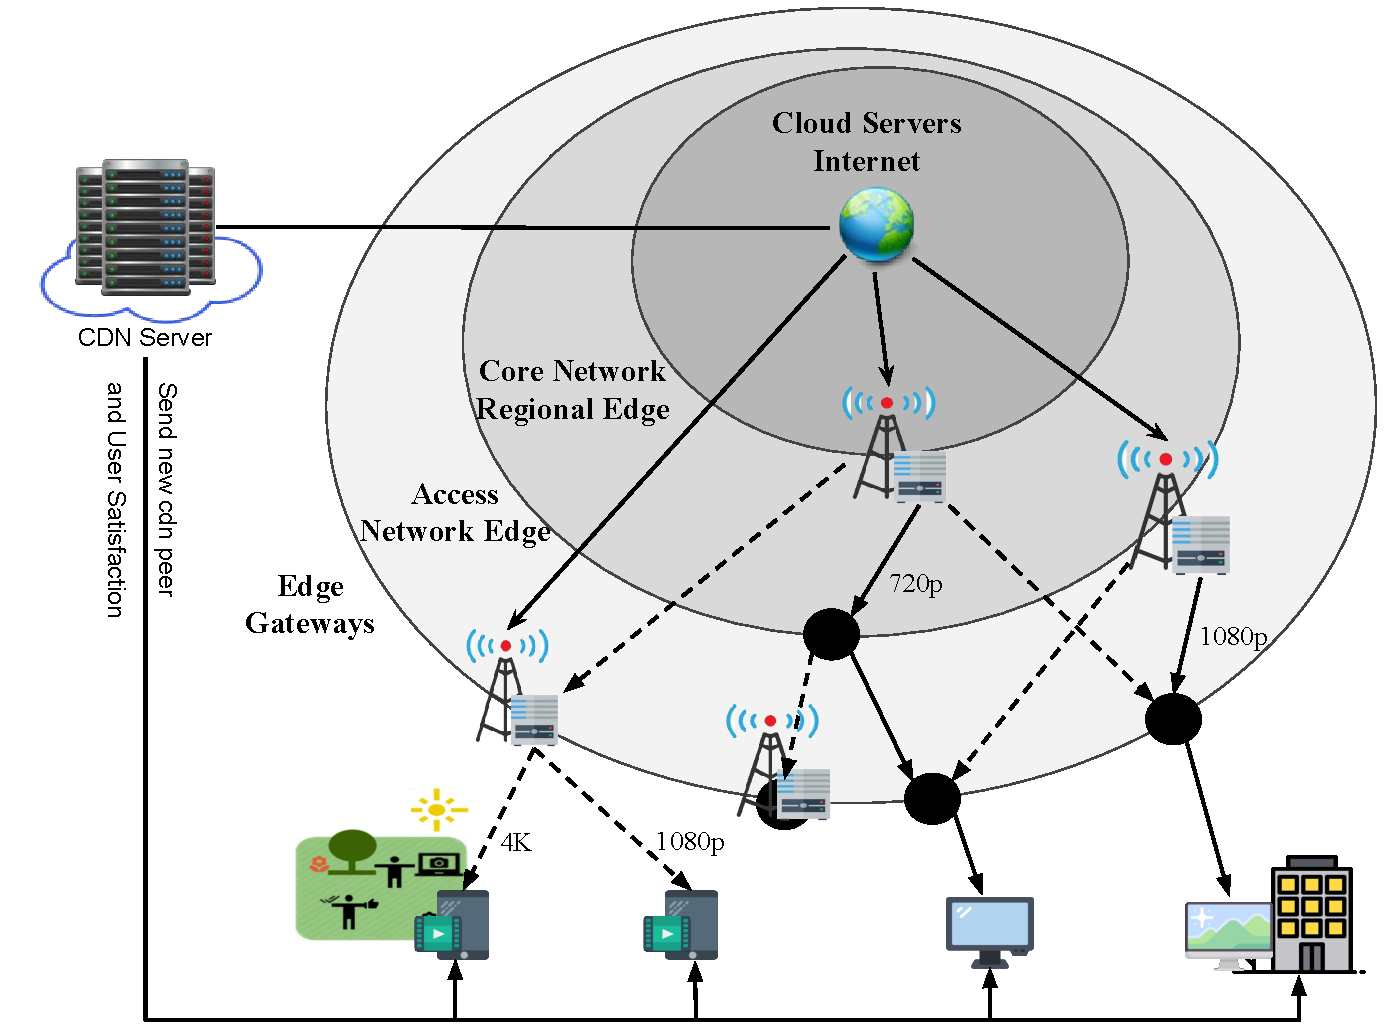
\includegraphics[width=0.9\linewidth]{images/arch-video-content.pdf}
    \caption{A General Overview of the multi-tier network environment.}
    \label{fig:multi-tier-network}
\end{figure}

% Objective
Motivated by these characteristics in multi-tier edge/cloud scenarios to improve users' satisfaction, as well as accommodate the growing video traffic. This article presents the need for an orchestrator in real-time to provide video streaming content.
Our goal is to provide designers and operators a performance analysis of a hierarchical edge network and its impacts on the users' QoE. The models we present in this paper are evaluated by a series of simulations using a controlled environment.

% Organization paper
This work is organized as follows.
Section \ref{sec:related-work} presents related work on the impact of edge/cloud networks on video streaming services.
Section \ref{sec:system-archi} briefly analysis the proposed multi-tier edge/cloud network and describe some opportunities of using such environments.
Section \ref{sec:results} shows preliminary results on the impact of the network performance for video streaming services.
Finally, \ref{sec:conclusion} concludes the paper.

\section{Motivation and Related Work}
\label{sec:related-work}

This section describes the related works in edge/cloud computing for video streaming. Here, some representative works in QoE are summarized regarding the edge network topologies and their impacts on video provisioning.

%CACA: Learning-based Content-aware Cache Admission for Video Content in Edge Caching
In Guan~\textit{et al.}~\cite{guan:2019:CLC} demonstrate the performance of the two-tier edge caching network. This work developed an algorithm to reach a 15\% of hit ratio in multimedia content consuming 20\% less memory usage. They deployed a video caching system. When a user requests a video, DNS-based mapping redirects the request to the nearest cache.
If the cache node does not hit the video, the edge node forwards it to the upper tier, which in turn forwards the request to the upper tier until it reaches the source. Otherwise, on any node storing the video in a cache, it will return immediately, and the current node will not forward the request to an upper tier.

Rosario~\textit{et al.}~\cite{rosarioSENSORS2018} present an architecture for virtual machine migration in real-time. During the migration, the video provisioning is moved forward over a multi-tier network. The architecture is based on the SDN paradigm for video distribution with QoE support. The work divides the edge into three tiers to ensure storage, upload and download capacity as presented in~\ref{fig:multi-tier-network}. In the experimental scenario, the cloud distributes the video content to the different edge levels with the multimedia service.

In Shen~\textit{et al.}~\cite{shenIWQoS19} works with a set of cache proxy services to analyze the cache miss occurrences. This work implements a reactive approach where cache proxies download the chunks of multimedia content when requested. The cache services use probability theory to improve the efficiency of transferring corresponding video segments in the cloud. In this way, they demonstrated an improvement in the users' QoE.

%Layered Hierarchical Caching for SVC-Based HTTP Adaptive Streaming over C-RAN
In Zhang~\textit{et al.}~\cite{zhang:WCNC2017}, the network consists of a cloud server connected to a pool of baseband units and a set of remote radio heads as cache nodes. The environment is organized hierarchically in multiple layers, where the proposed heuristic is formulated to consider the download rate between the nodes in the cache. The solution has two objectives: to minimize the amount of backhaul traffic and to improve the hit rate in VoD systems

Bentaleb~\textit{et al.}~\cite{bentaleb:2018:MSys} develop a Game Theory Algorithm (GTA), a new customer-oriented scheme whithin client-side that seeks to select the best bitrate. Unlike most works in DASH Multimedia Systems, in which users strive to maximize the QoE of the viewer without considering other entities on the network, this solution allows efficient collaboration between different player entities. The GTA improves the users' QoE with emphasis on the perceptual quality of the viewer, without explicit communication overload, respecting the decision requirements of the existing players. In addition, this work considers the cross-traffic in different network conditions.

%In this project we aim to design a video delivery system that considers such issues to improve quality of experience for a range of video streaming needs, including low latency requirements.
The approaches above could decrease the traffic load and improve QoE. However, more issues arise in such dynamic scenarios: user mobility, collaborative cache services over multi-edge, users' number during flash crowds, and interactive streaming requirements are not fully considered.  Proper management and orchestration of video delivery over the Internet is core to the smooth coexistence of heterogeneous video services. This work focus on edge/cloud hierarchy to show the impacts of video streaming services in a multi-tier environment, as well as the need to have a real-time video streaming orchestration.

%The aforementioned approaches could decrease the traffic load and improve QoE, but more
%issues arise in such scenarios: user mobility, collaborative cache schemes over multi-edge, the amount of users during flash crowds, and interactive streaming requirements are not fully considered. In this project we aim to design a video delivery system that considers such issues to improve quality of experience for a range of video streaming needs, including low latency requirements.
%
%
%The aforementioned approaches could decrease the traffic load and improve QoE, but more
%issues arise in such scenarios: user mobility, collaborative cache schemes over multi-edge, the amount of users during flash crowds, and interactive streaming requirements are not fully considered. In this project we aim to design a video delivery system that considers such issues to improve quality of experience for a range of video streaming needs, including low latency requirements.

\section{Analysing and Opportunities of a Video Streaming Architecture}
\label{sec:system-archi}

%{\color{blue} This section explains the architecture system, and what it is  for, explaining some protocols flowcharts. Studying the protocols and focusing in the system part of the experiments.}

%This section explains the modeling used in our experiments. We first provide an overview of the proposed video streaming service impacts in multi-tier networks. The remaining subsections describe the implementation of this service architecture.
To design a cache hierarchies on vertically organized edge nodes with N tiers presents some improvements in users' QoE. The before-mentioned architecture can achieve such advantages by serving the requested content as close as possible to the user. So that efficiently forwarding requests between parent edge nodes within the hierarchy, balancing the video traffic in terms of hop counts and users attended. In addition, the network core congestion is reduced since it represents an operational overhead for the content provider.
As a preliminary outcome achieved by a multi-tier network experiment, the QoE impact over a video streaming service is assessed. Thereafter, we describe some facts about the QoE characteristics and insights on the opportunities of caching multimedia content in edge nodes of multi-tier networks.

\subsection{Impact of Fog Multi-tier Network Approach}

To confirm these differences in users' performance requesting a video from cache nodes in different tiers, we present two users requesting multimedia content in different layers. Then an analysis of the impacts over the network is addressed. The Figure~\ref{fig:impact-two-layers} illustrates a two-tier network model, the graphs show the results of bitrate, interruptions, buffer and representations switch, respectively, from left to right.%and along x-axis the simulation time. 
When a client requests a cache edge node video, it can be located in layer L1 or L2. Where each layer level has different network factors, e.g., load, latency, so on. Accordingly the Figure~\ref{fig:multi-tier-network}, an L1 layer can be interpreted as a personal computer, laptops, and smartphones, where the node retransmits the video content through wired or wireless communication. Whereas in the L2 layer a specific Edge gateway can be distributed on local edge nodes, for example.

\begin{figure}
    \centering
    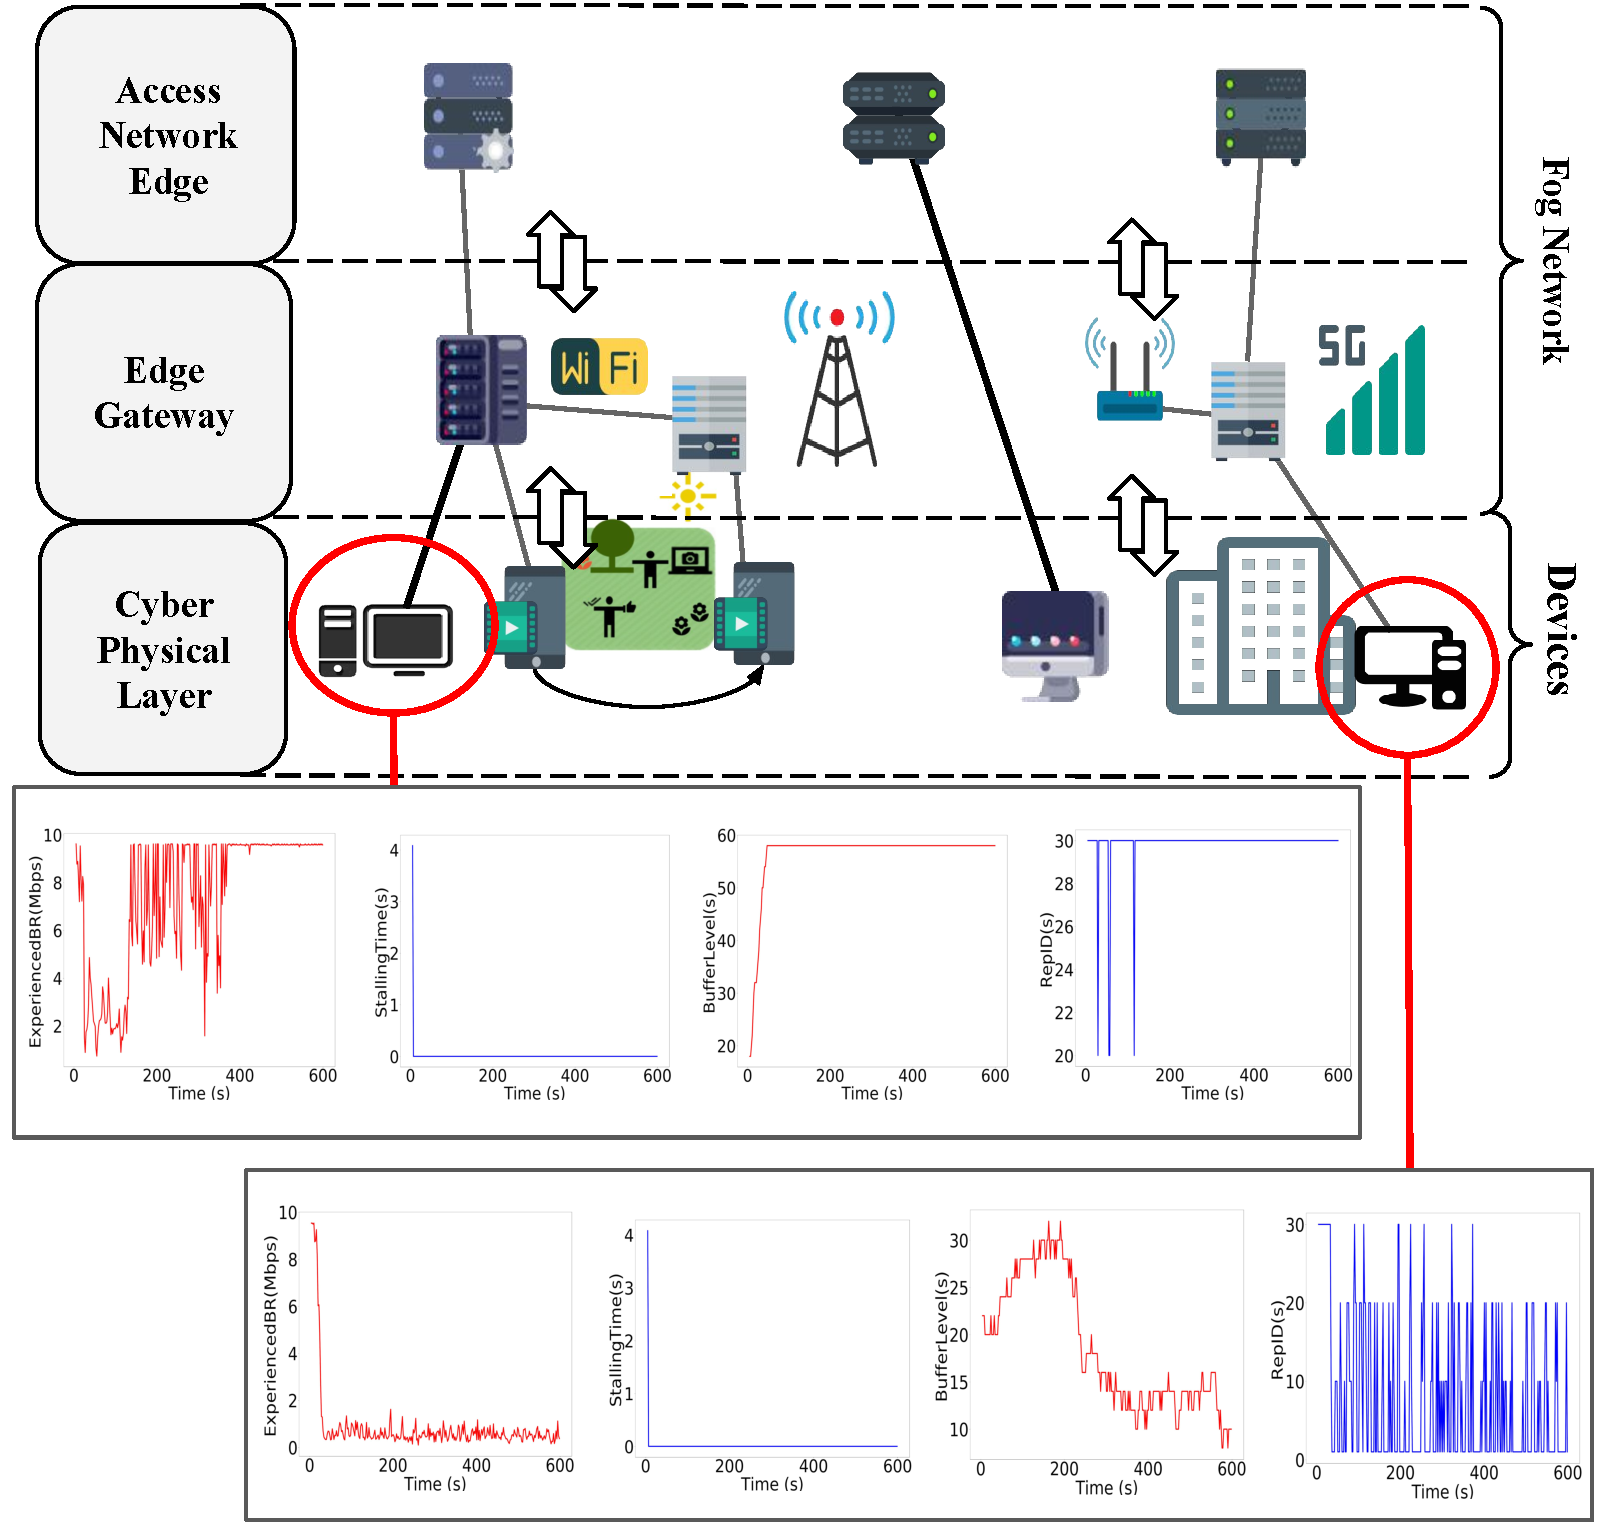
\includegraphics[width=0.9\linewidth]{images/qoe-multi-level.pdf}
    \caption{\textbf{The number of bitrate switches, stalls, buffer size, the startup delay in seconds of a DASH player requesting a video with 10 bitrate levels varying from 50 to 4,500Kbps and from nodes in different tiers.}}
    \label{fig:impact-two-layers}
\end{figure}


As we can see, besides the initial interruption until the start of the video, both users have had no interruptions throughout the video execution. However, the user who received the video on the nearest edge layer had a higher bit rate than the other user. As well as the buffer was soon filled and the user had the best possible resolution of the video. Whereas the user who received the video from a distant layer, in some moments, worked with the buffer at the limit and had to constantly switch resolutions so that there is no interruption during the video execution. Both users received a same from different Layers, even without any interruptions during the video transmission, differnet layers impacts directly the users' QoE.


\subsection{Multi-tier Edge-Cloud Network Opportunities}

%Esta seção apresenta algumas oportunidades dentro de redes multi-tier edge/cloud para o provisionamento da transmissção de videos. Aproveitar nós próximos aos usuários podem melhorar o funcionamento do rede como um todo, aqui nós discutimos alguns insights que podem ser usados em favor dos stakeholders que utilizam a infraestrutura para transmissão de video. 
The opportunities within multi-tier edge/cloud networks for the provision of video transmission is presented. Taking advantage of nodes close to users can improve the functioning of the network as a whole, here we discuss some insights that can be used in favor of network and provider admin who use the infrastructure for video transmission.

\subsubsection{Improving User QoE}

%the cloud distributes the video content to the different levels of the edge. Depending the level which the video is cached the users' experience changes. The architecture is based on held the video distribution with QoE support. The work divides the edge into three layers, to guarantee coverage, storage, upload and download capacity. 
Inside a multi-tier environment composed of more than one domain of devices, the domain resources can host the video content near the end-users, reducing latency and mitigating the load on the network's core. The fog nodes are composed of specific resources combined to carry out the video transmission to integrate video streaming services in such communication environments. Within this context, mechanisms for integrating schemes and video streaming raise as an opportunity to improve QoE.% at each network level.
The results reported in Fig~\ref{fig:impact-two-layers} shows that it is possible to improve the users' satisfaction using the edge multi-tier network. Depending on the level of allocation of the video service, the video smoothing variation between characteristics of the player changes.


\subsubsection{Potential Bandwith Saving}

%Video Caching, Analytics, and Delivery at the Wireless Edge: A Survey and Future Directions
Videos streamed in higher quality increase network bandwidth. Consequently, provisioning from the Cloud will incur high communication expenses. 
The process of delivering part of the video along the network can significantly save bandwidth utilization instead of sending all frames to the edge server or by lowering the encoding quality of uninteresting portions of the frames. Different delivery approaches can have different performances to reduce the uplink bandwidth. Moreover, none of the surveyed articles have considered the end-to-end design of video streaming, wherein the edge server adapts the video streams based on uplink and downlink bandwidth capacities. Additionally, new forms of video content are being generated today.


\subsubsection{Cacheability}

Caching audio/video during peak hours ...
Manage the QoE users refer to those services where the Controller can centrally control the satisfaction guarantees. The Controller can address this problem by creating a control channel to managed-quality video streaming services over the edge-cloud network.


\section{Performance Evaluation}
\label{sec:results}

This section describes the experimental evaluation of the strategy proposed to redirect the users, including the scenarios, metrics, methodology, and outcomes.
 
%\subsection{Methodology}
%
%We present three approaches to address the methodological problems identified in a edge/cloud multi-tier network for watching a video streaming: cloud-only 

\subsection{Experimental Setup}

%[29] Christian Kreuzberger, Daniel Posch, and Hermann Hellwagner. Amust framework - adaptive multimedia streaming simulation framework for ns-3 and ndnsim, 2016.
%[30] C. Mueller, S. Lederer, J. Poecher, and C. Timmerer. Demo paper: Libdash - an open source software library for the mpeg-dash standard. In 2013 IEEE International Conference on Multimedia and Expo Workshops (ICMEW), pages 1–2, July 2013.
% Per-title encode optimization, 2015. ; accessed 20-novembro-2019.

We use Adaptive Multimedia Streaming~(AMuSt)~\cite{kreuzberger2016amust} to implement a video streaming server, and the server is implemented through Dynamic Adaptive Streaming over HTTP~(DASH) and users that allow adaptive video streaming. The AMuSt framework provides a set of applications for producing and consuming adaptable videos based on the DASH standard. DASH functionality is provided by the libdash library~\cite{mueller2013ICMEW}, an open source library that provides an interface to the DASH standard. Currently, libdash is the official reference software for the DASH standard. We consider that users are interested in an available video with ten different bit rate representations \{235kbps, 375kbps, 560kbps, 560kbps, 750kbps, 1050kbps, 1750kbps, 2350kbps, 3000kbps, 4300kbps, 5800kbps\}, which are used by Netflix subsets~\cite{netflix:representation}, which Netflix uses. [31]. Each representation is divided into 2-second segments. Each experiment is executed once with a video of 1600 seconds~(800 segments). 
For the sake of simplicity, the multimedia content used in the simulation is already deployed in the edge peering nodes. 

%Figure 3 shows the topology with three levels used in the experiments, each level \{1, 2 and 3\} is represented as a scenario.

%Dash server and the clients allowed to request a multimedia content in DASH format, was used the Adaptive Multimedia Streaming~(AMuSt). The AMust system allow a set o apps to produce and consume the adaptive video, based on Dash pattern. The DASH functionality is provided by the libdash library, an open source library that provides an interface to the DASH standard. Currently, libdash is the reference software official DASH standard.

We simulate the scenario in a binary tree topology with seven nodes and a Cloud Provider connected to the root node of the Binary tree. The last four nodes are Access Points~(AP), and the others are edge peering points. Figure~\ref{fig:exp-setup-scenario} illustrate the binary tree scenario.

The AP nodes are implemented on a wireless device that communicates via IEEE 802.11g in 2.4GHz frequency. The APs are connected to the edge peering points by wire and the end-users via wireless. Each user connected to the AP is located precisely 8 meters away. The Bandwidth available in each link can seem in Fig.~\ref{fig:exp-setup-scenario}.

We present three approaches to address the impacts identified in Section~\ref{sec:system-archi} into the edge/cloud multi-tier network: the \textit{cloud-only}, \textit{1\&2 nodes} and mobile-based scenarios. The cloud-only scenario uses just the Cloud Provider node to deliver the video content. \textit{1\&2 nodes} uses nodes 1 and 2 as auxiliary nodes to deliver the video. The simulation starts with the users requesting the video from the cloud. When some link detects a congested link, the edge cache below the link is turned on. Thereafter, the users receiving the video over the congested link are redirected to the edge node. 

The number of end-user devices communicating through each wireless AP may change over time due to the mobility of the end-user devices. In practice, the number of end-user devices connecting to the wireless AP changes frequently. 
To show the problems that can appear in such scenarios, and a connection change between the APs occurs. We reran the second experiment, maintaining connections between users and edge nodes, but changed the connection between users and APs. Where half the users of each $AP_{i}$ go directly to $AP_{i + 2}$.
%Onde os metade dos usuários de cada $AP_{i}$ vão diretamente para o $AP_{i+2}$.
%Para mostrar os problemas que podem aparecer em tais cenários, e ocorre uma mudança de conexão entre os APs. Nós executamos novamente o segundo experimento mantendo as conexões entre os usuários e edge nodes, mas mudamos a conexão entre os usuários e os APs. 


\begin{figure}
    \centering
    %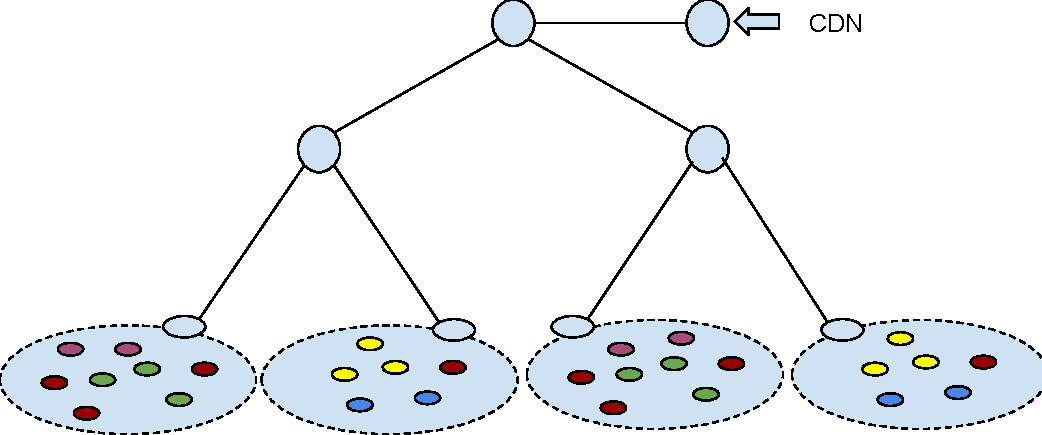
\includegraphics[width=0.9\linewidth]{images/exp-setup-scenario.pdf}
    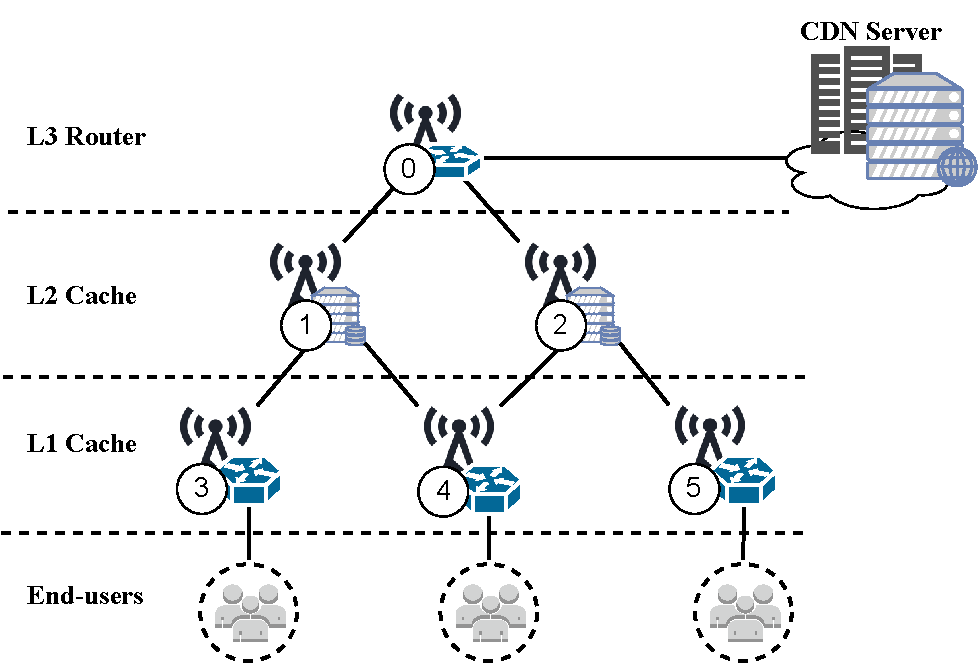
\includegraphics[width=\linewidth]{images/qoe-multi-level-2.pdf}
    \caption{A General Overview of the multi-tier network environment.}
    \label{fig:exp-setup-scenario}
\end{figure}

%To illustrate the idea, we assume tree topology. According to the guideline, a mobile backhaul network is modeled as a two-level hierarchical network. Wireless base stations are connected to aggregation nodes, e.g., service/packet data network gateway (S/P-GW) nodes. Furthermore, aggregation nodes are connected to core nodes, e.g., central office nodes. To the best of our knowledge, separation of traffic from one wireless base stations to multiple aggregation nodes, and from one aggregation node to multiple core nodes is not dominant in current mobile backhaul networks. Thus, we assume a tree-topology backhaul network


\subsection{QoE Metric evaluation}

There exist many viewer QoE models in the literature. We will describe the QoE metrics used to score user satisfaction. Firstly, We compute each video quality chunk by a logarithmic law over bitrates~\cite{Reichl:TSys2013}. The study proposes a video quality model for DASH, as shown in Equation (1). Each video has $N$ segments and is encoded with $L$ bitrate levels. $r_i$ represents a specific bitrate level. At each step $i$, the quality of segment $i$, which is encoded at $l_i$ is defined as:

$$
q(r_i) = a_1 * log(a_2 * (r_i/ r_{|L|}))
$$

We require a flexible QoE model that includes the most influential metrics to quantify long-term users' QoE. 
We consider the Eq.~\ref{eq:qoe-equation} which consists of four metrics: (a) the average chunk perceptual quality, (b) the average number of quality oscillations, (c) the average number of stall events and their durations, and (d) the startup delay. $K$ represents the total segments of the video, $S_{i}$ is the stall duration, and $ST_{i}$ is the startup delay of user $i$.

\begin{equation}\label{eq:qoe-equation}
\begin{split}
QoE_i = \frac{1}{K} \sum_{k=1}^{K}q(r_{k}) - \frac{1}{K-1} \sum_{k=1}^{K-1}|q(r_{k+1}) - q(r_{k}))| \\
- \frac{1}{K}\sum_{k=1}^{K} S_{k} - ST_{i}
\end{split}
\end{equation}

The $QoE_{i}$ for each user $i$ has a range of 1 to 5. Where the values 1 = bad, 2 = poor, 3 = fair, 4 = good, and 5 = excellent.

%
% \begin{figure*}
%     \centering
%     \subfigure[]{
%     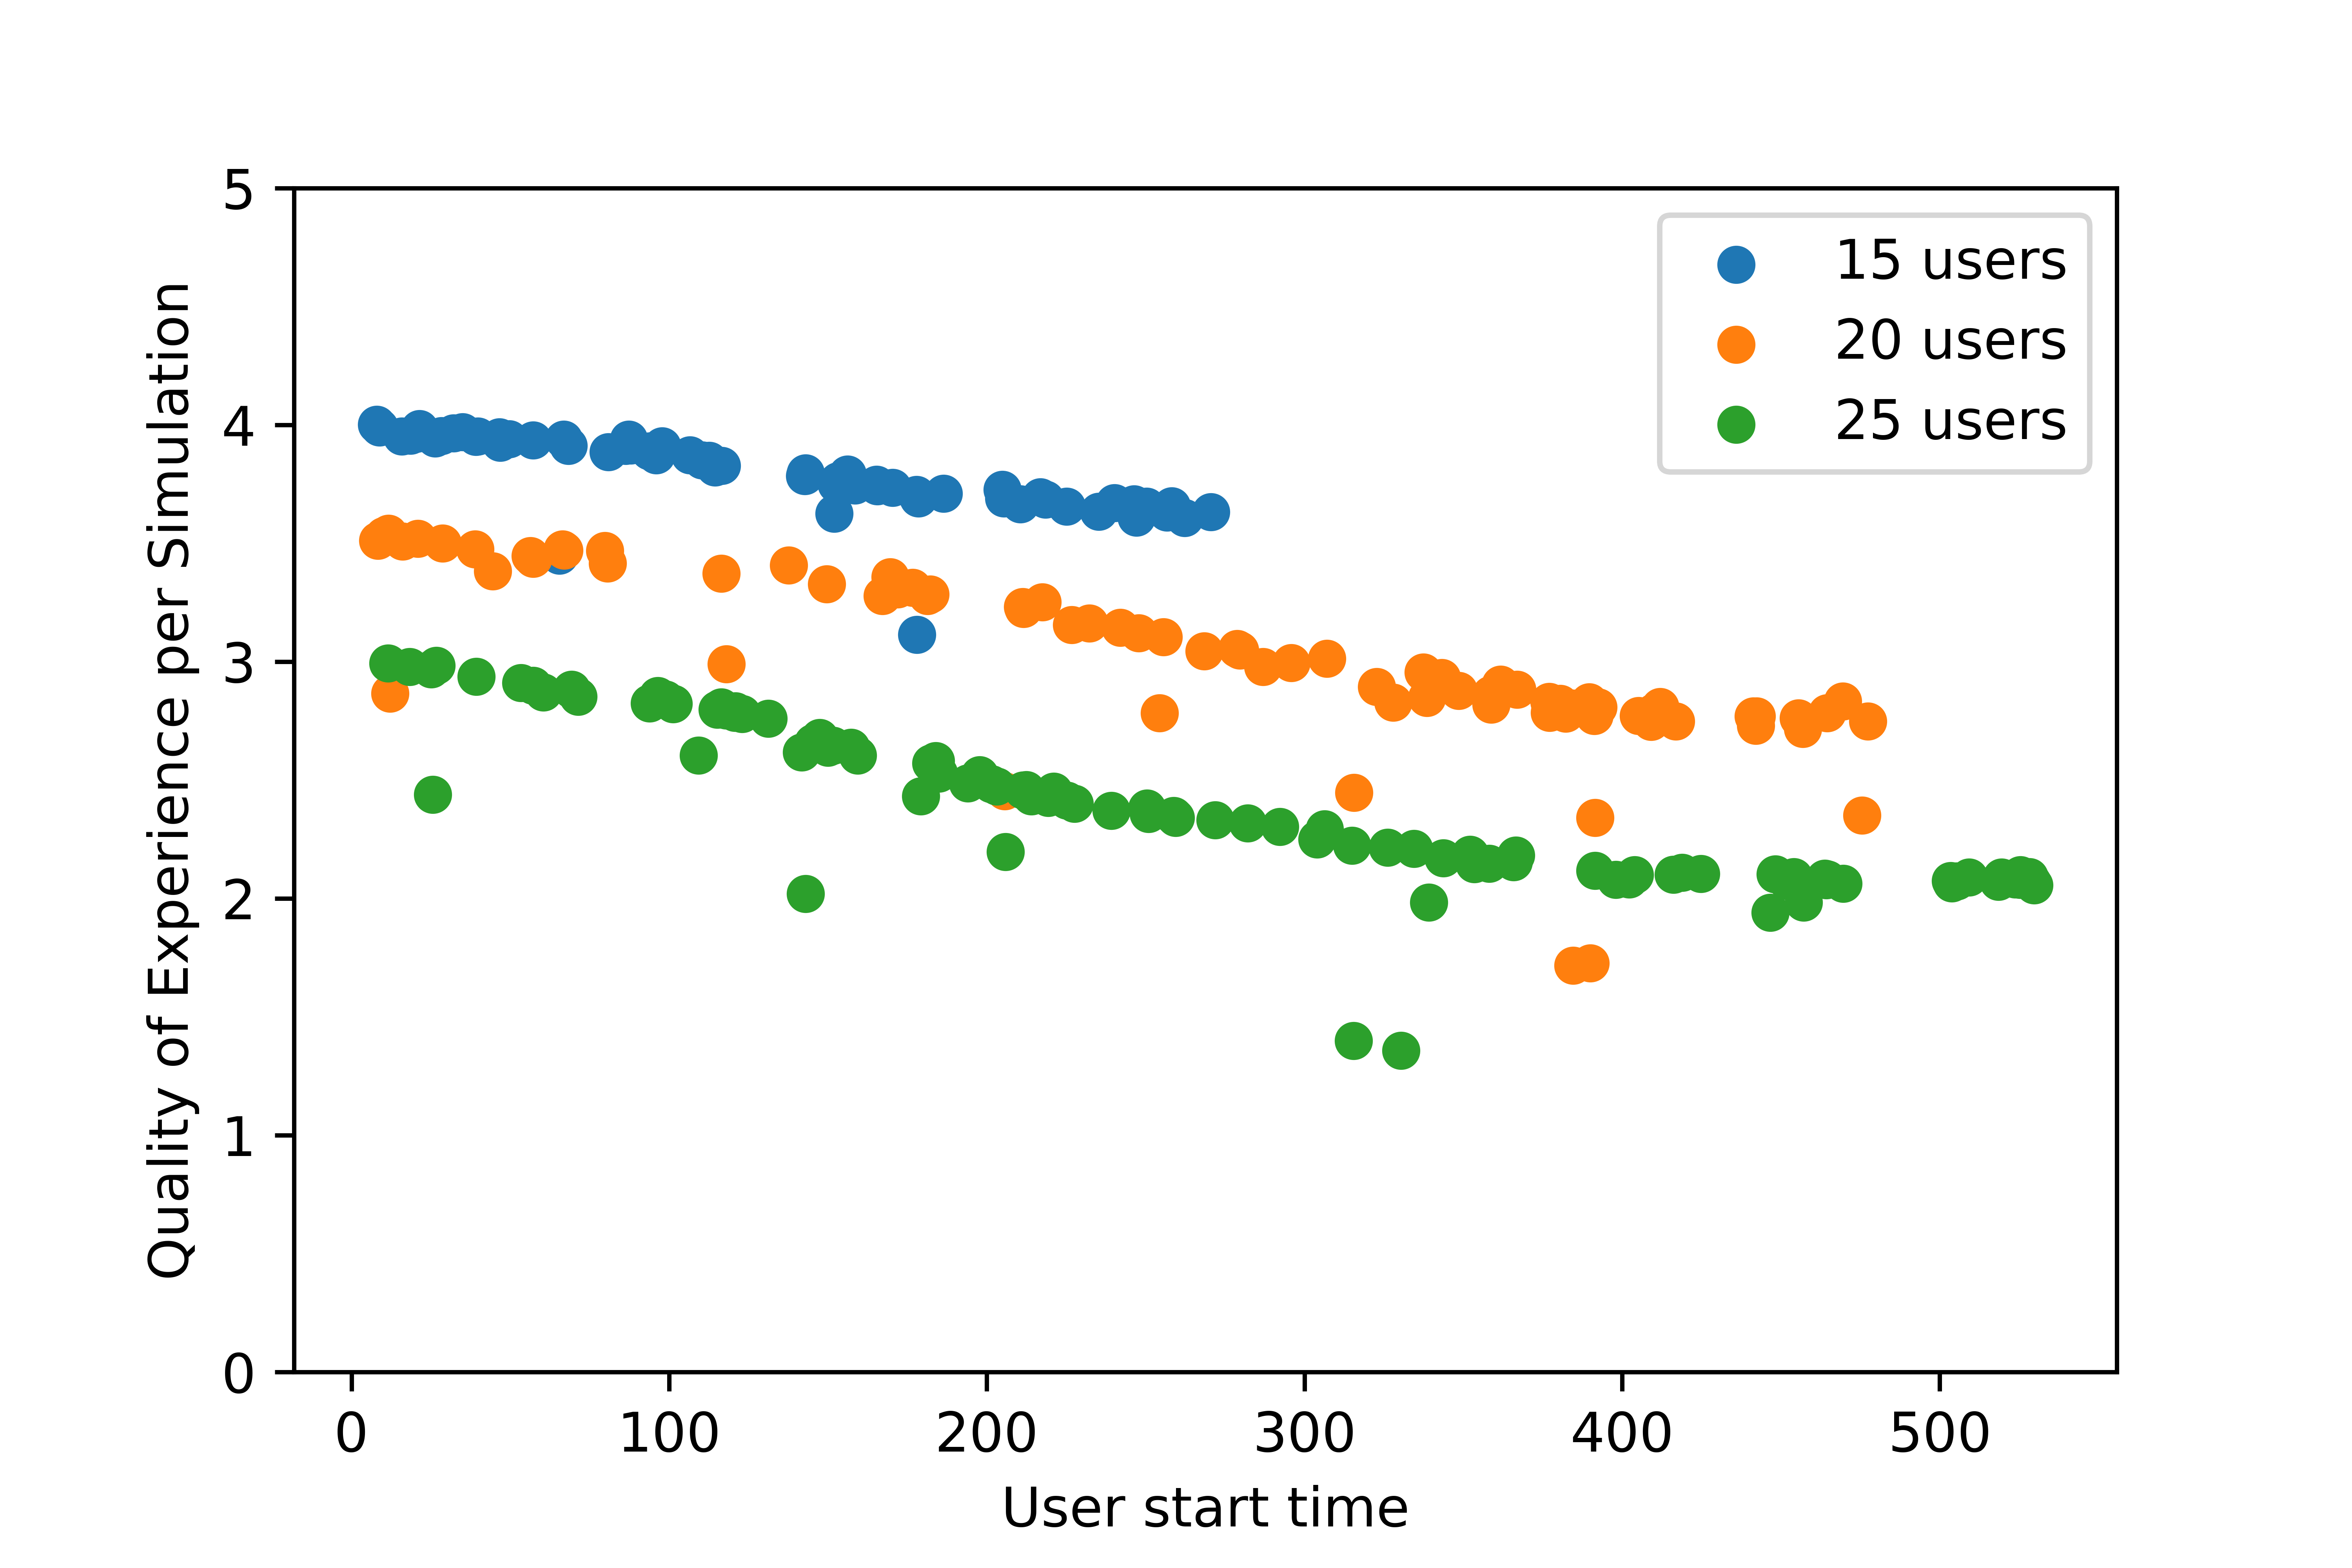
\includegraphics[width=0.45\linewidth]{images/QoECompare.png}
%     \label{fig:red-comparison-plot}
%     }
%     \subfigure[]{
%     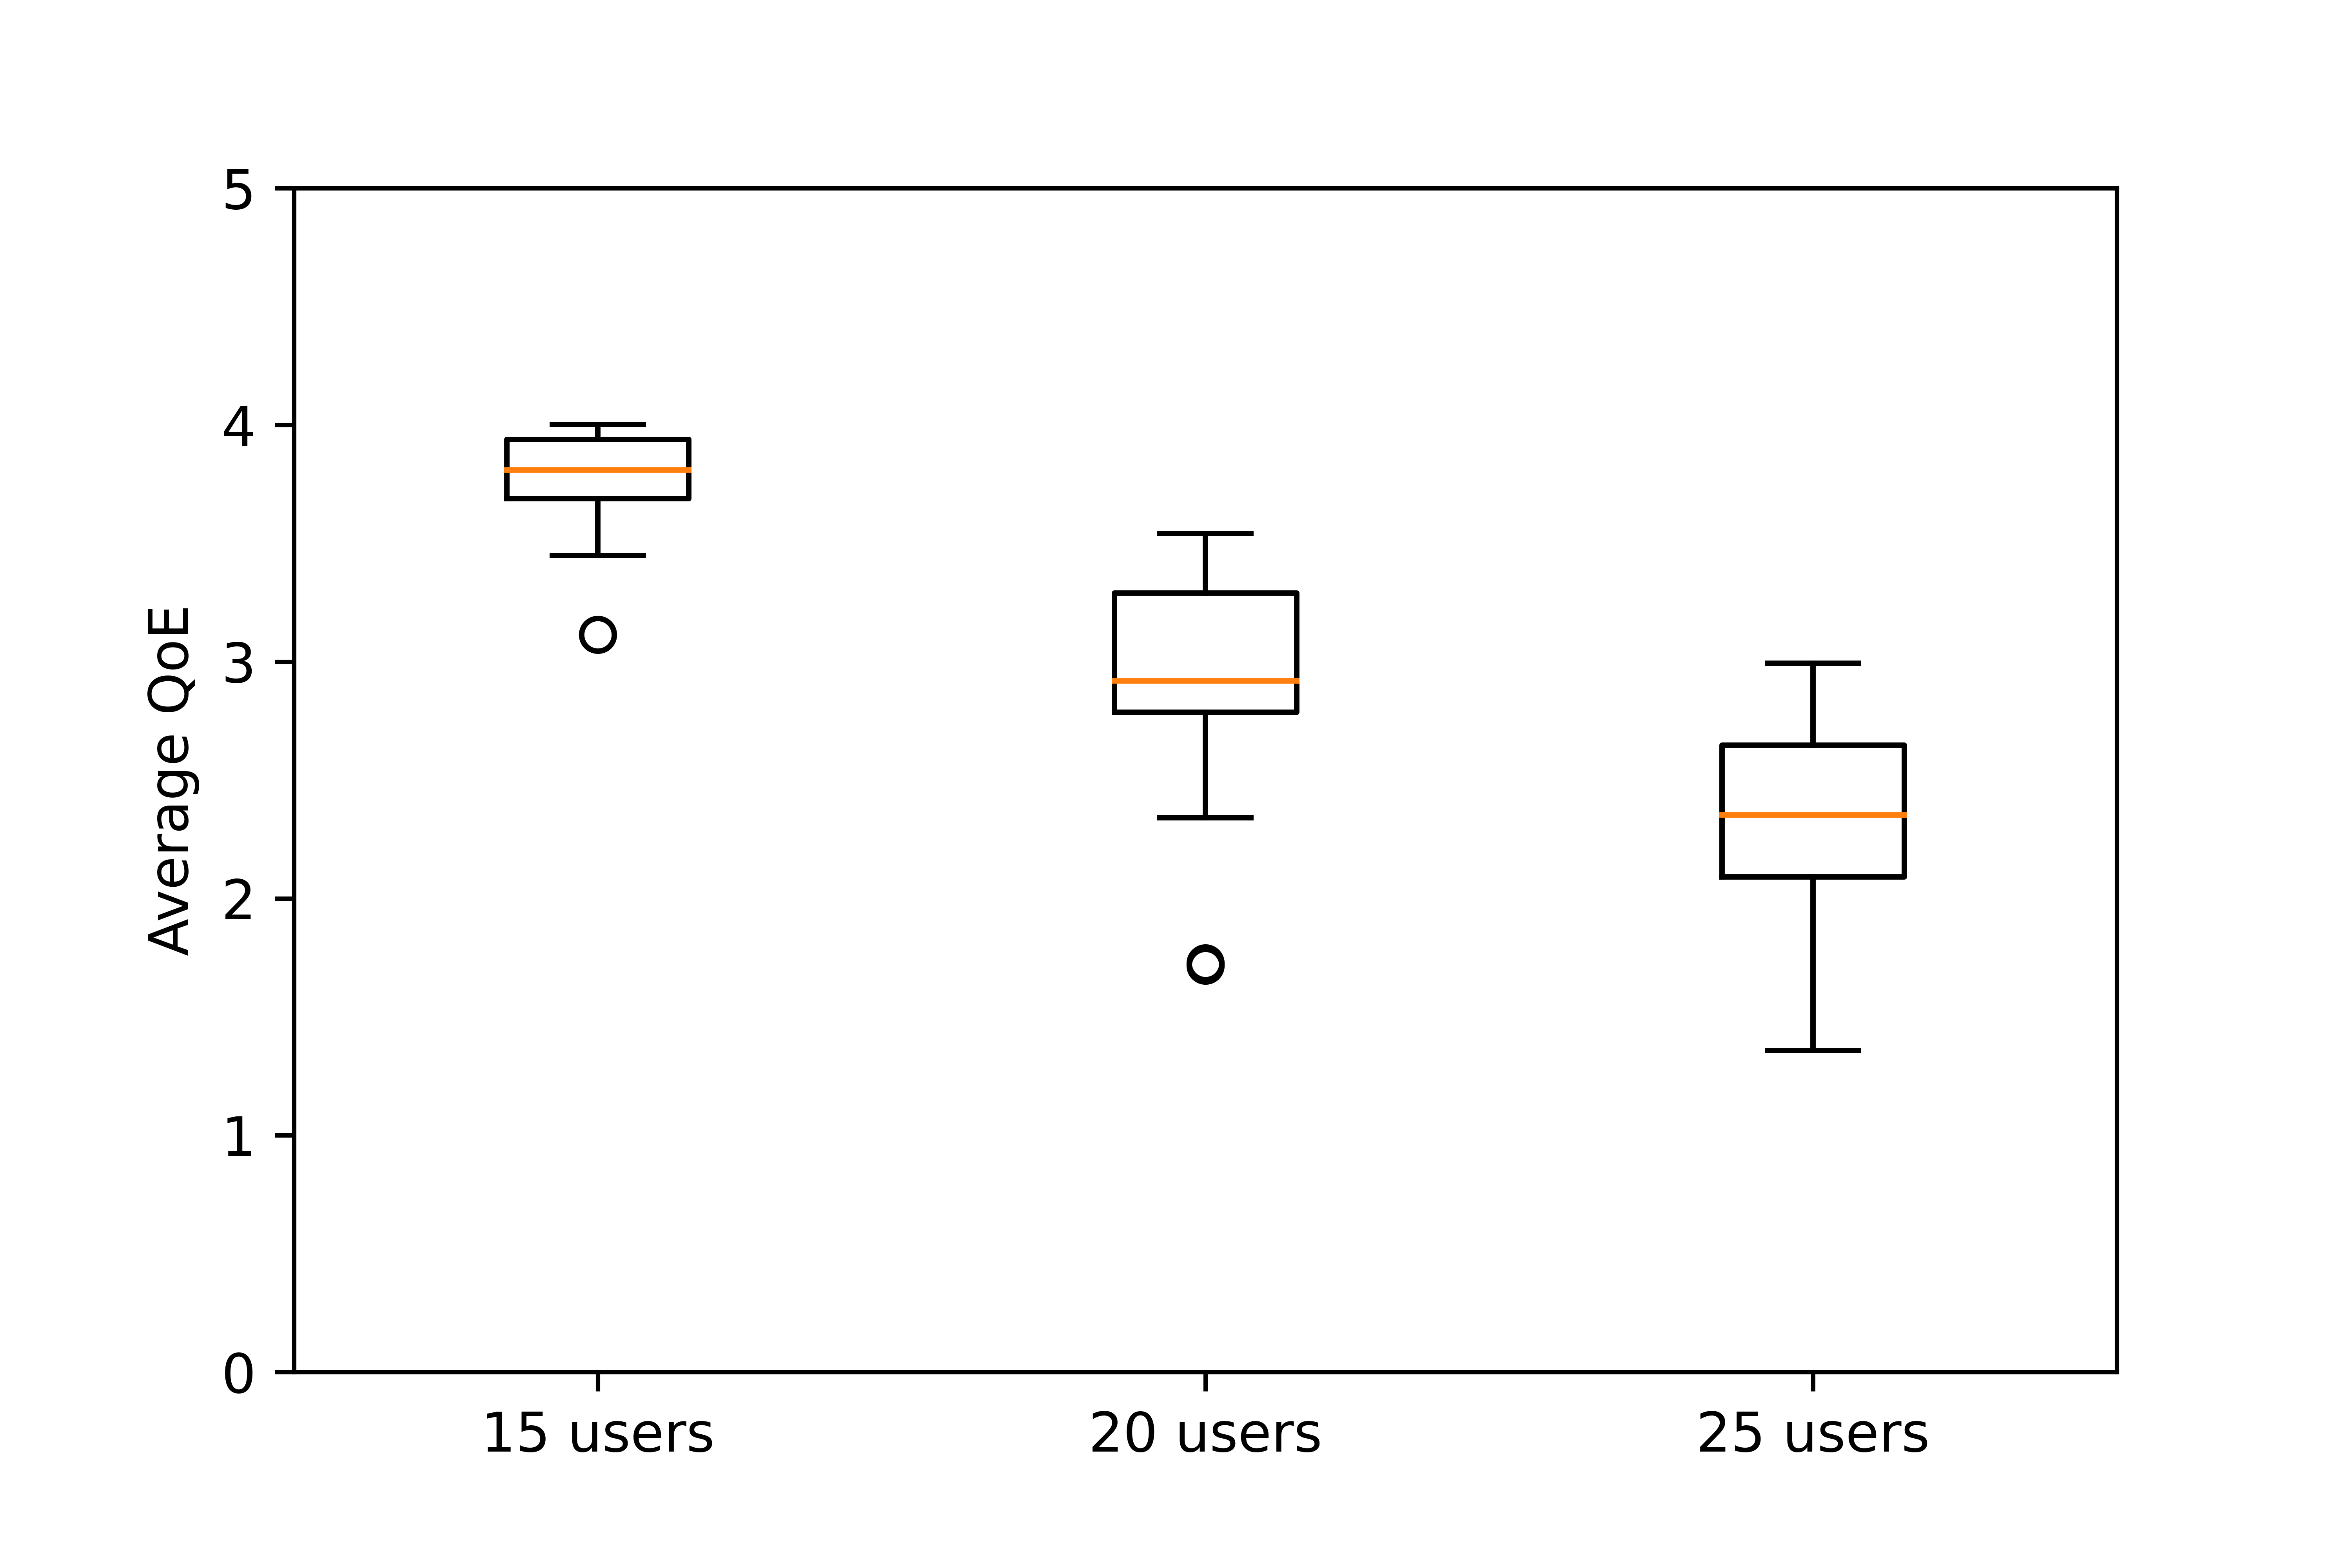
\includegraphics[width=0.45\linewidth]{images/QoEBoxplot.png}
%     \label{fig:co-comparison-boxplot}
%     }

%     \subfigure[]{
%     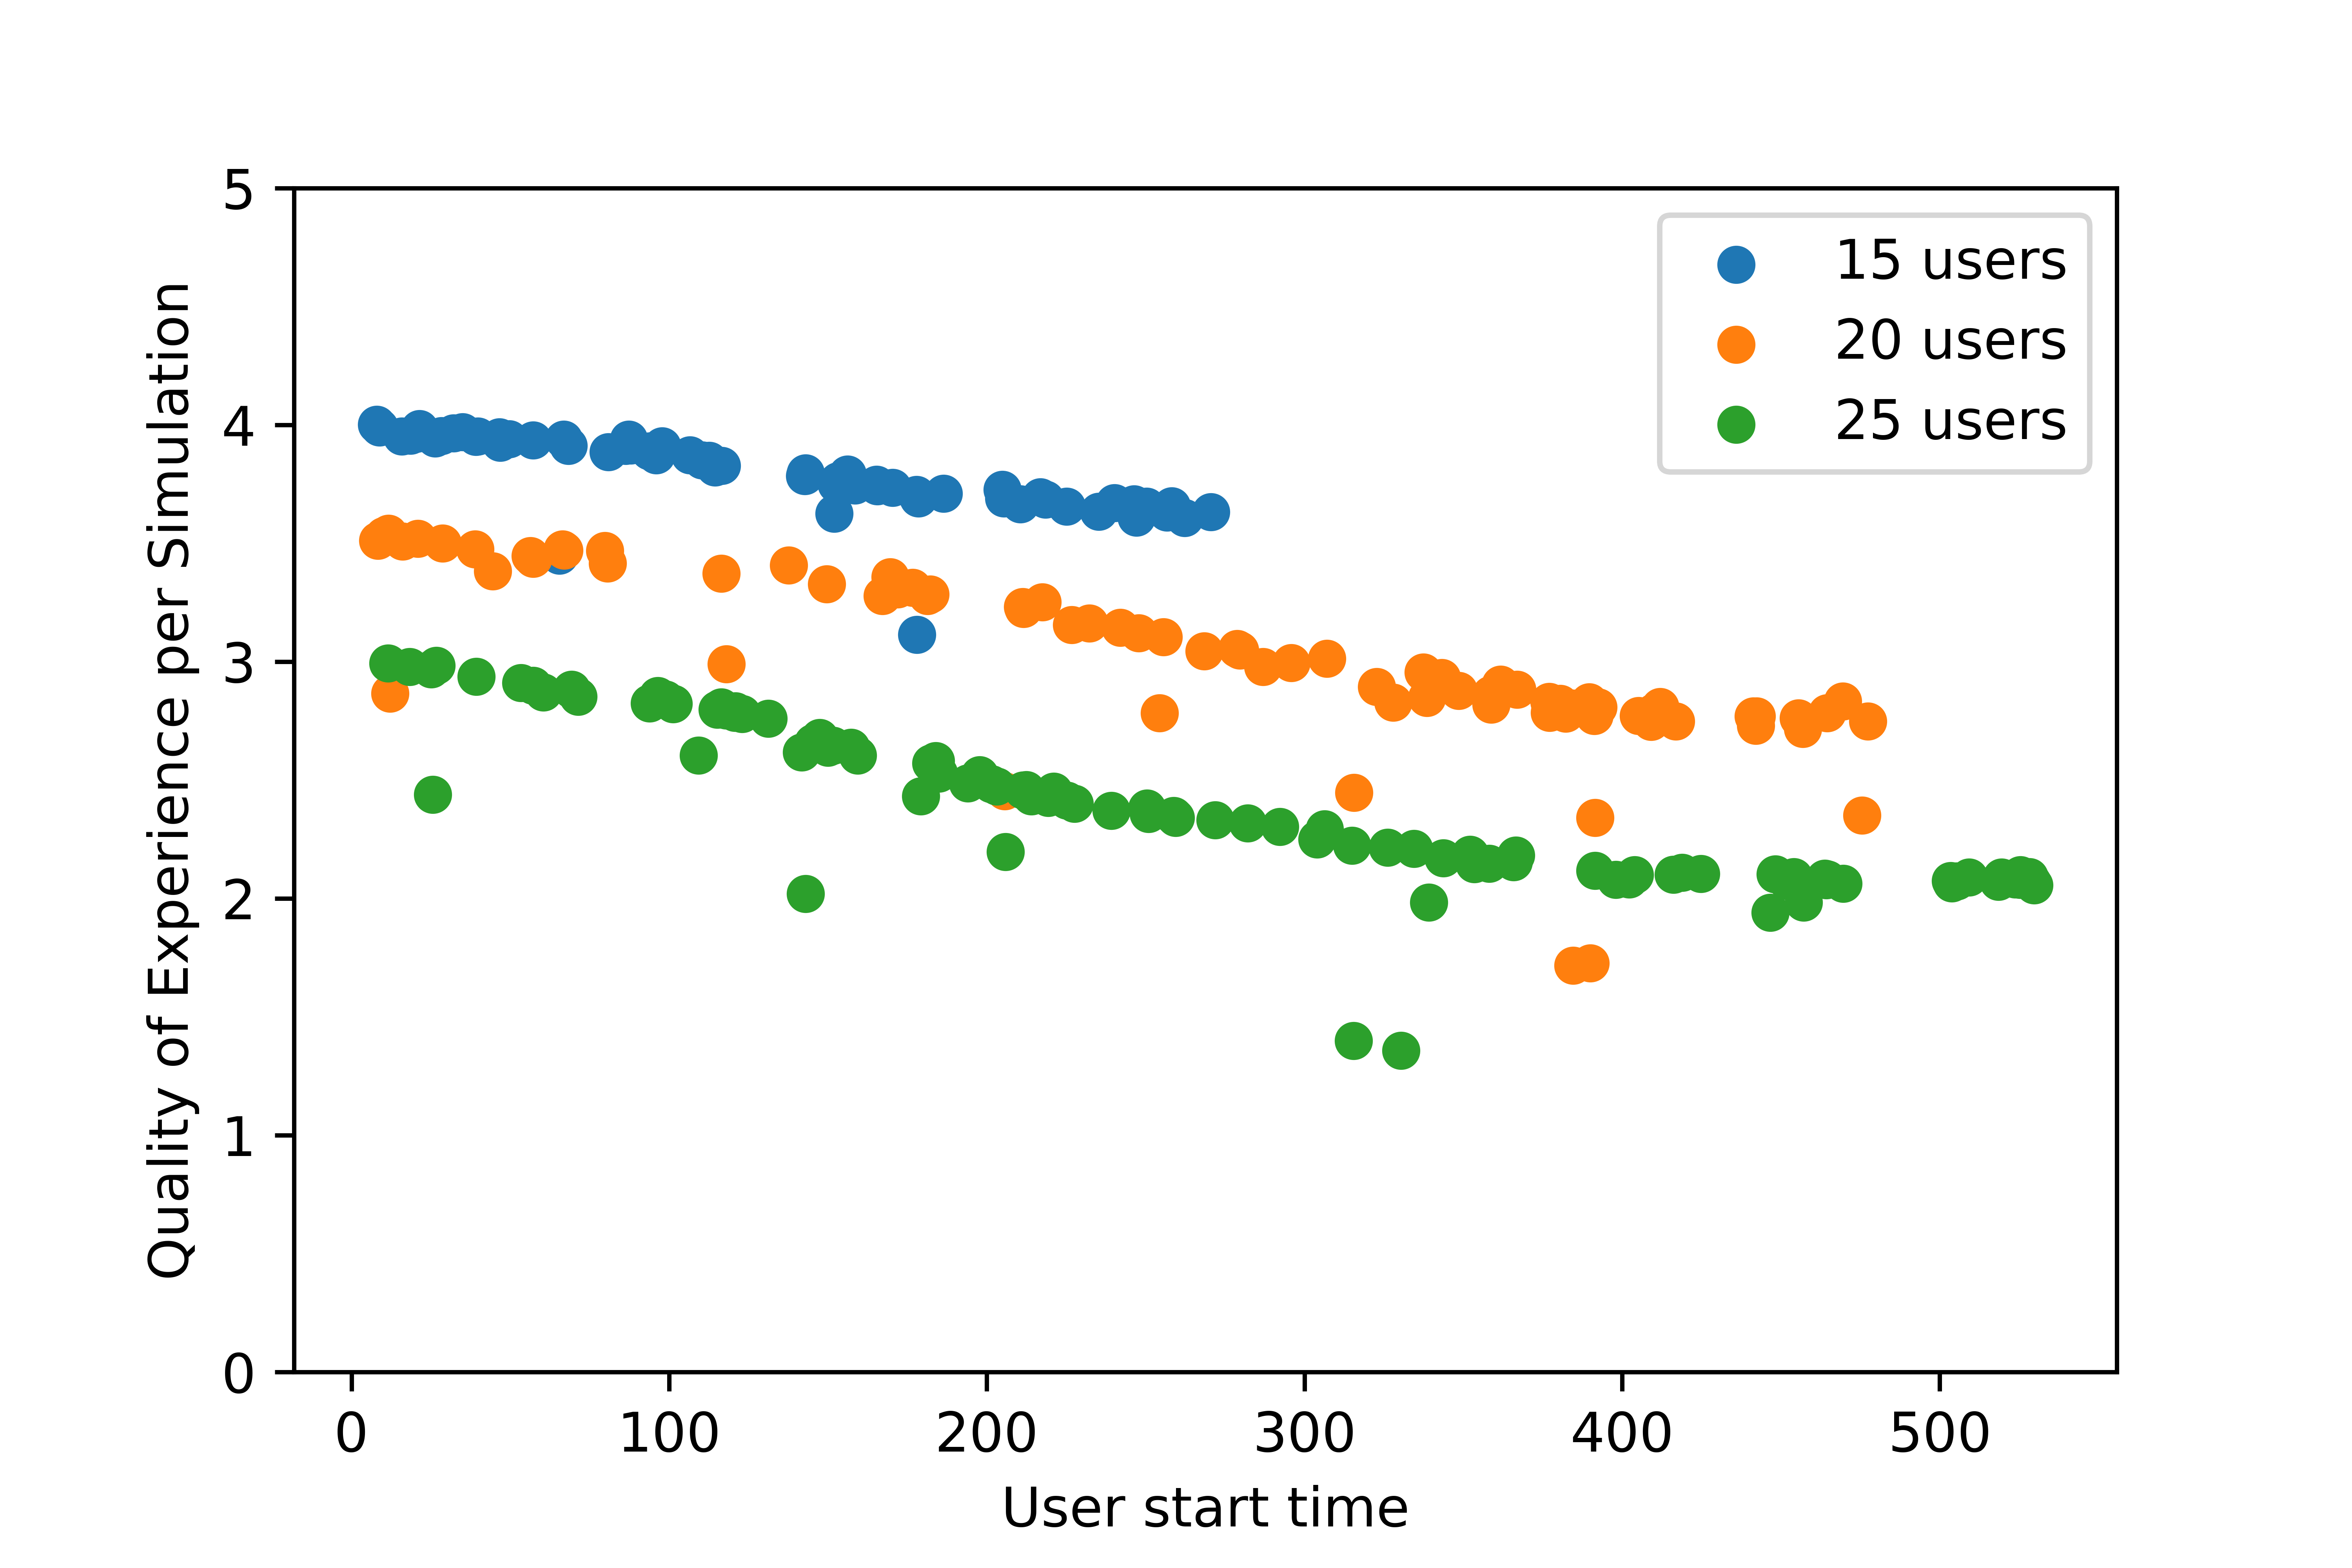
\includegraphics[width=0.45\linewidth]{images/QoECompare.png}
%     \label{fig:red-comparison-plot}
%     }
%     \subfigure[]{
%     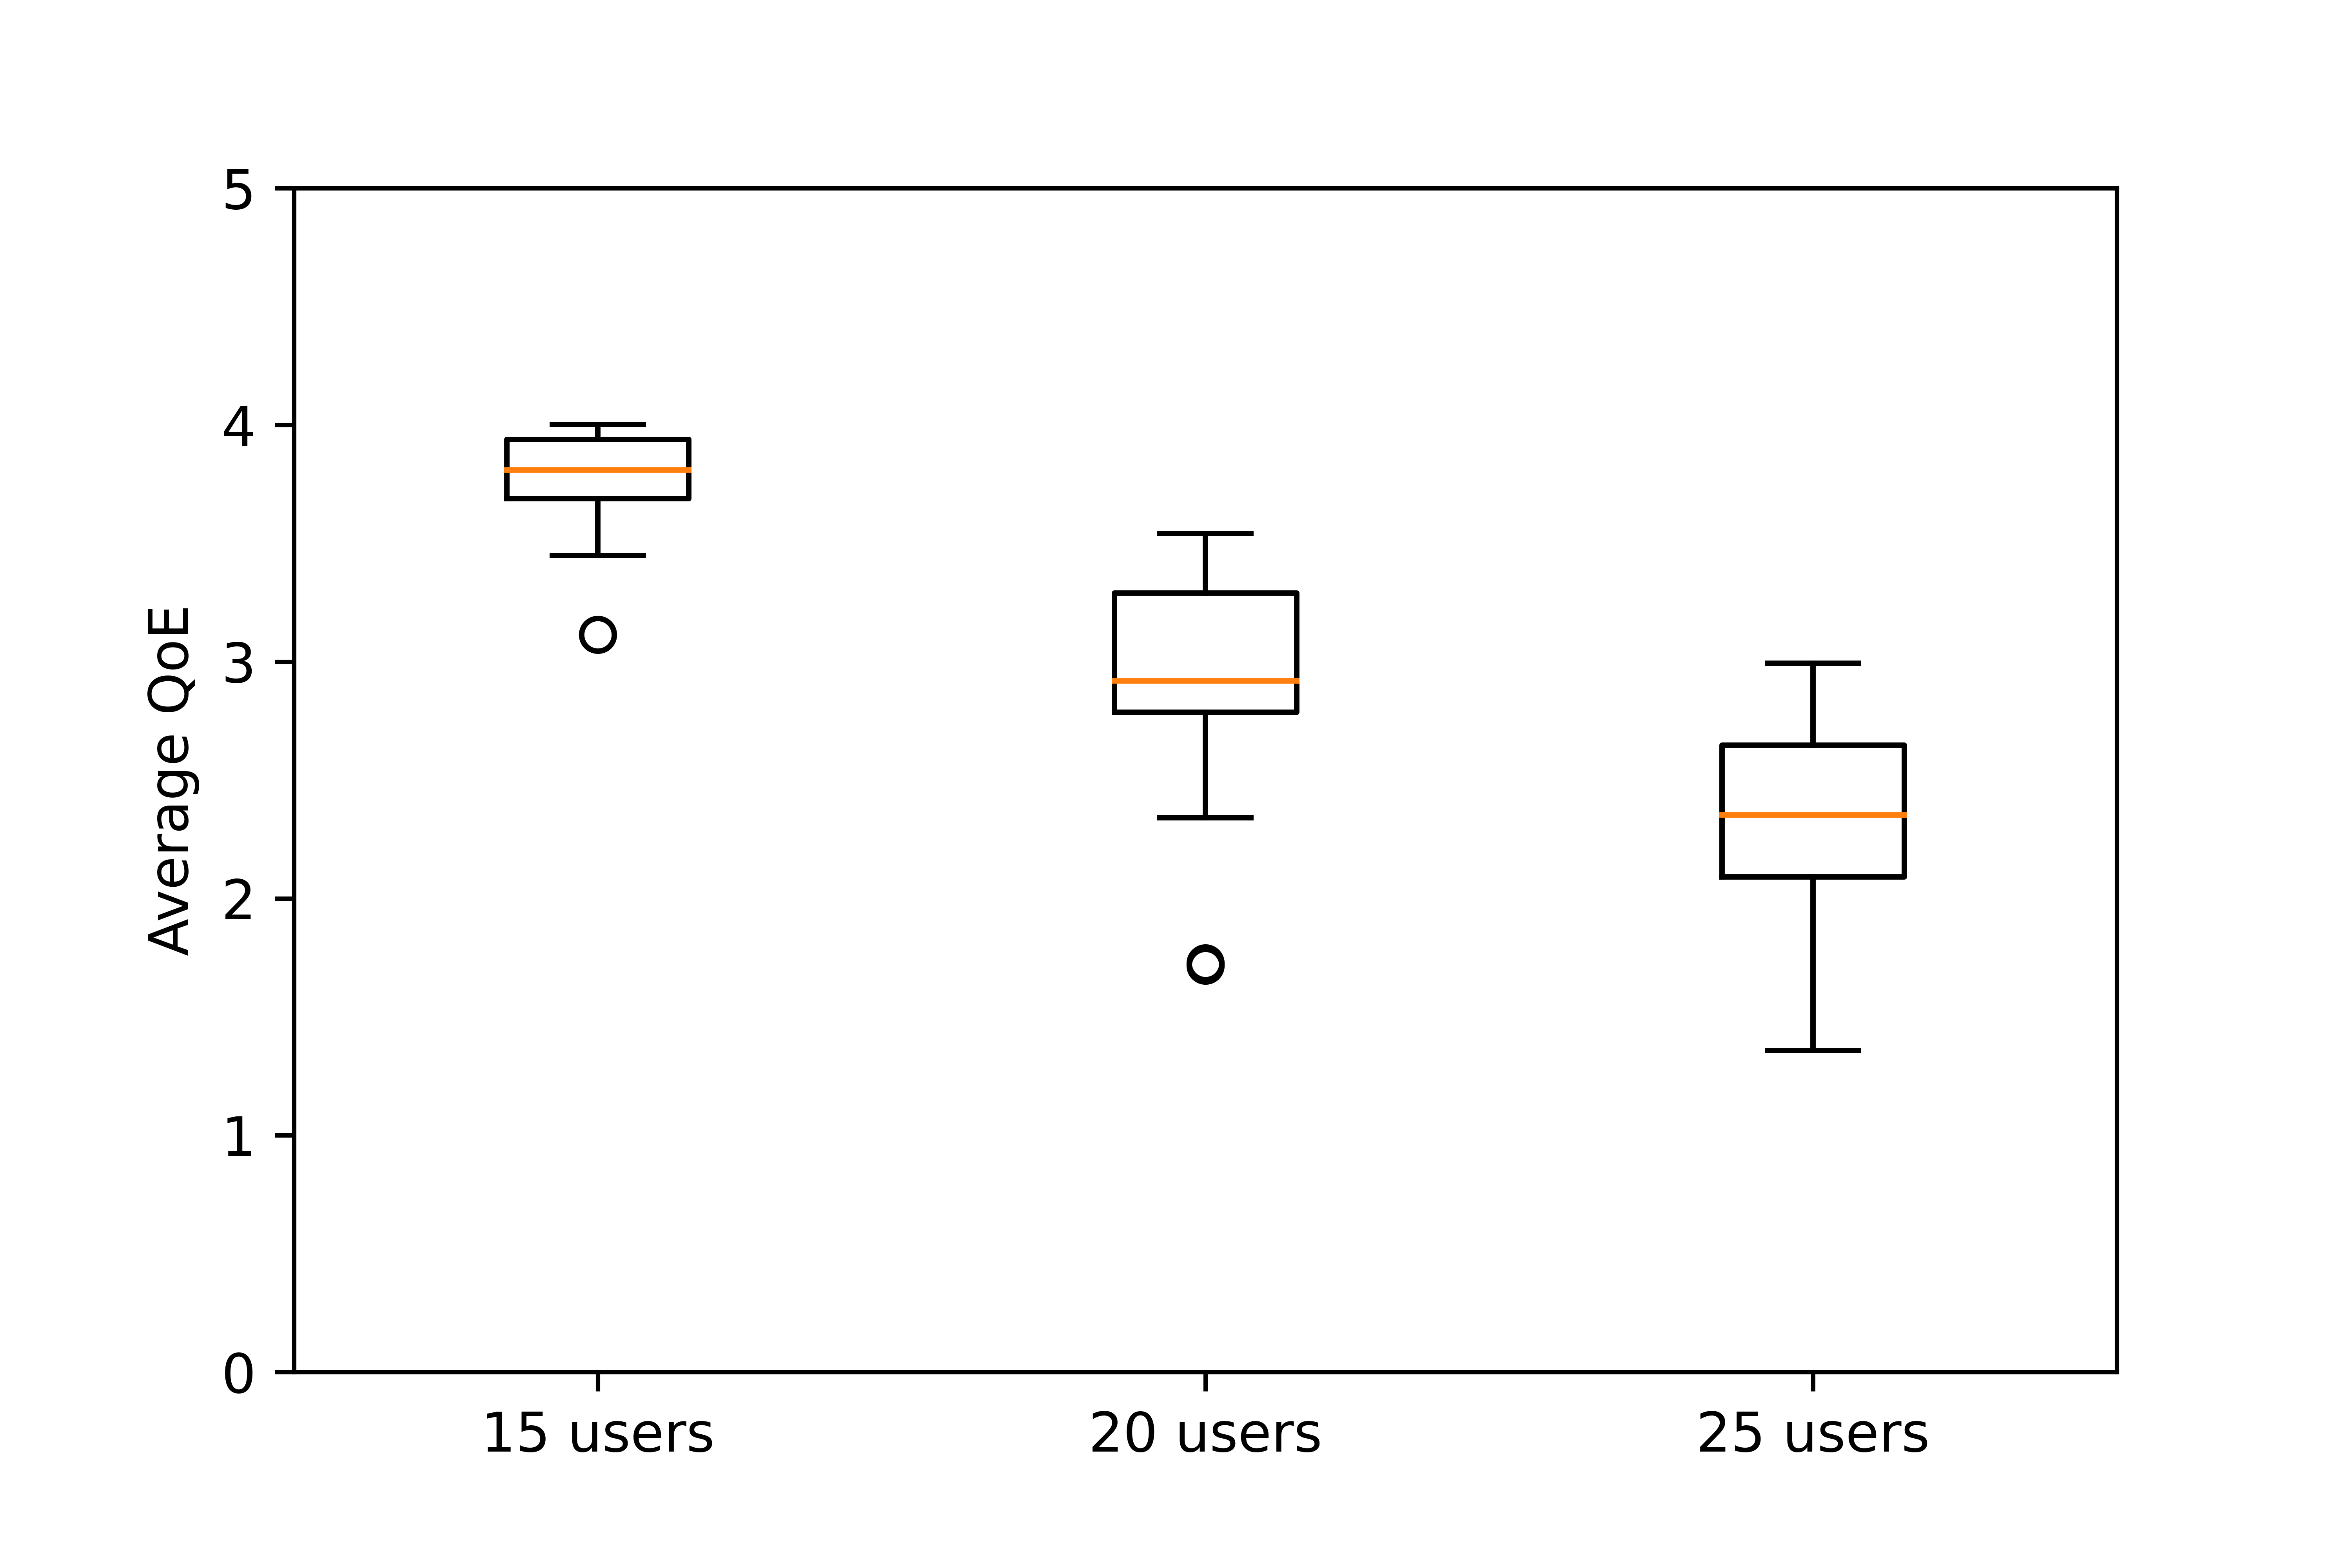
\includegraphics[width=0.45\linewidth]{images/QoEBoxplot.png}
%     \label{fig:red-comparison-boxplot}
%     }

%     \caption{Impact of system on the network performance. Distance \textit{d} between sensor node and antennas of 8m in a semi-NLOS scenario.}
%     \label{fig:comparison-rof-2}
% \end{figure*}

\begin{figure*}
    \centering
    \subfigure[]{
    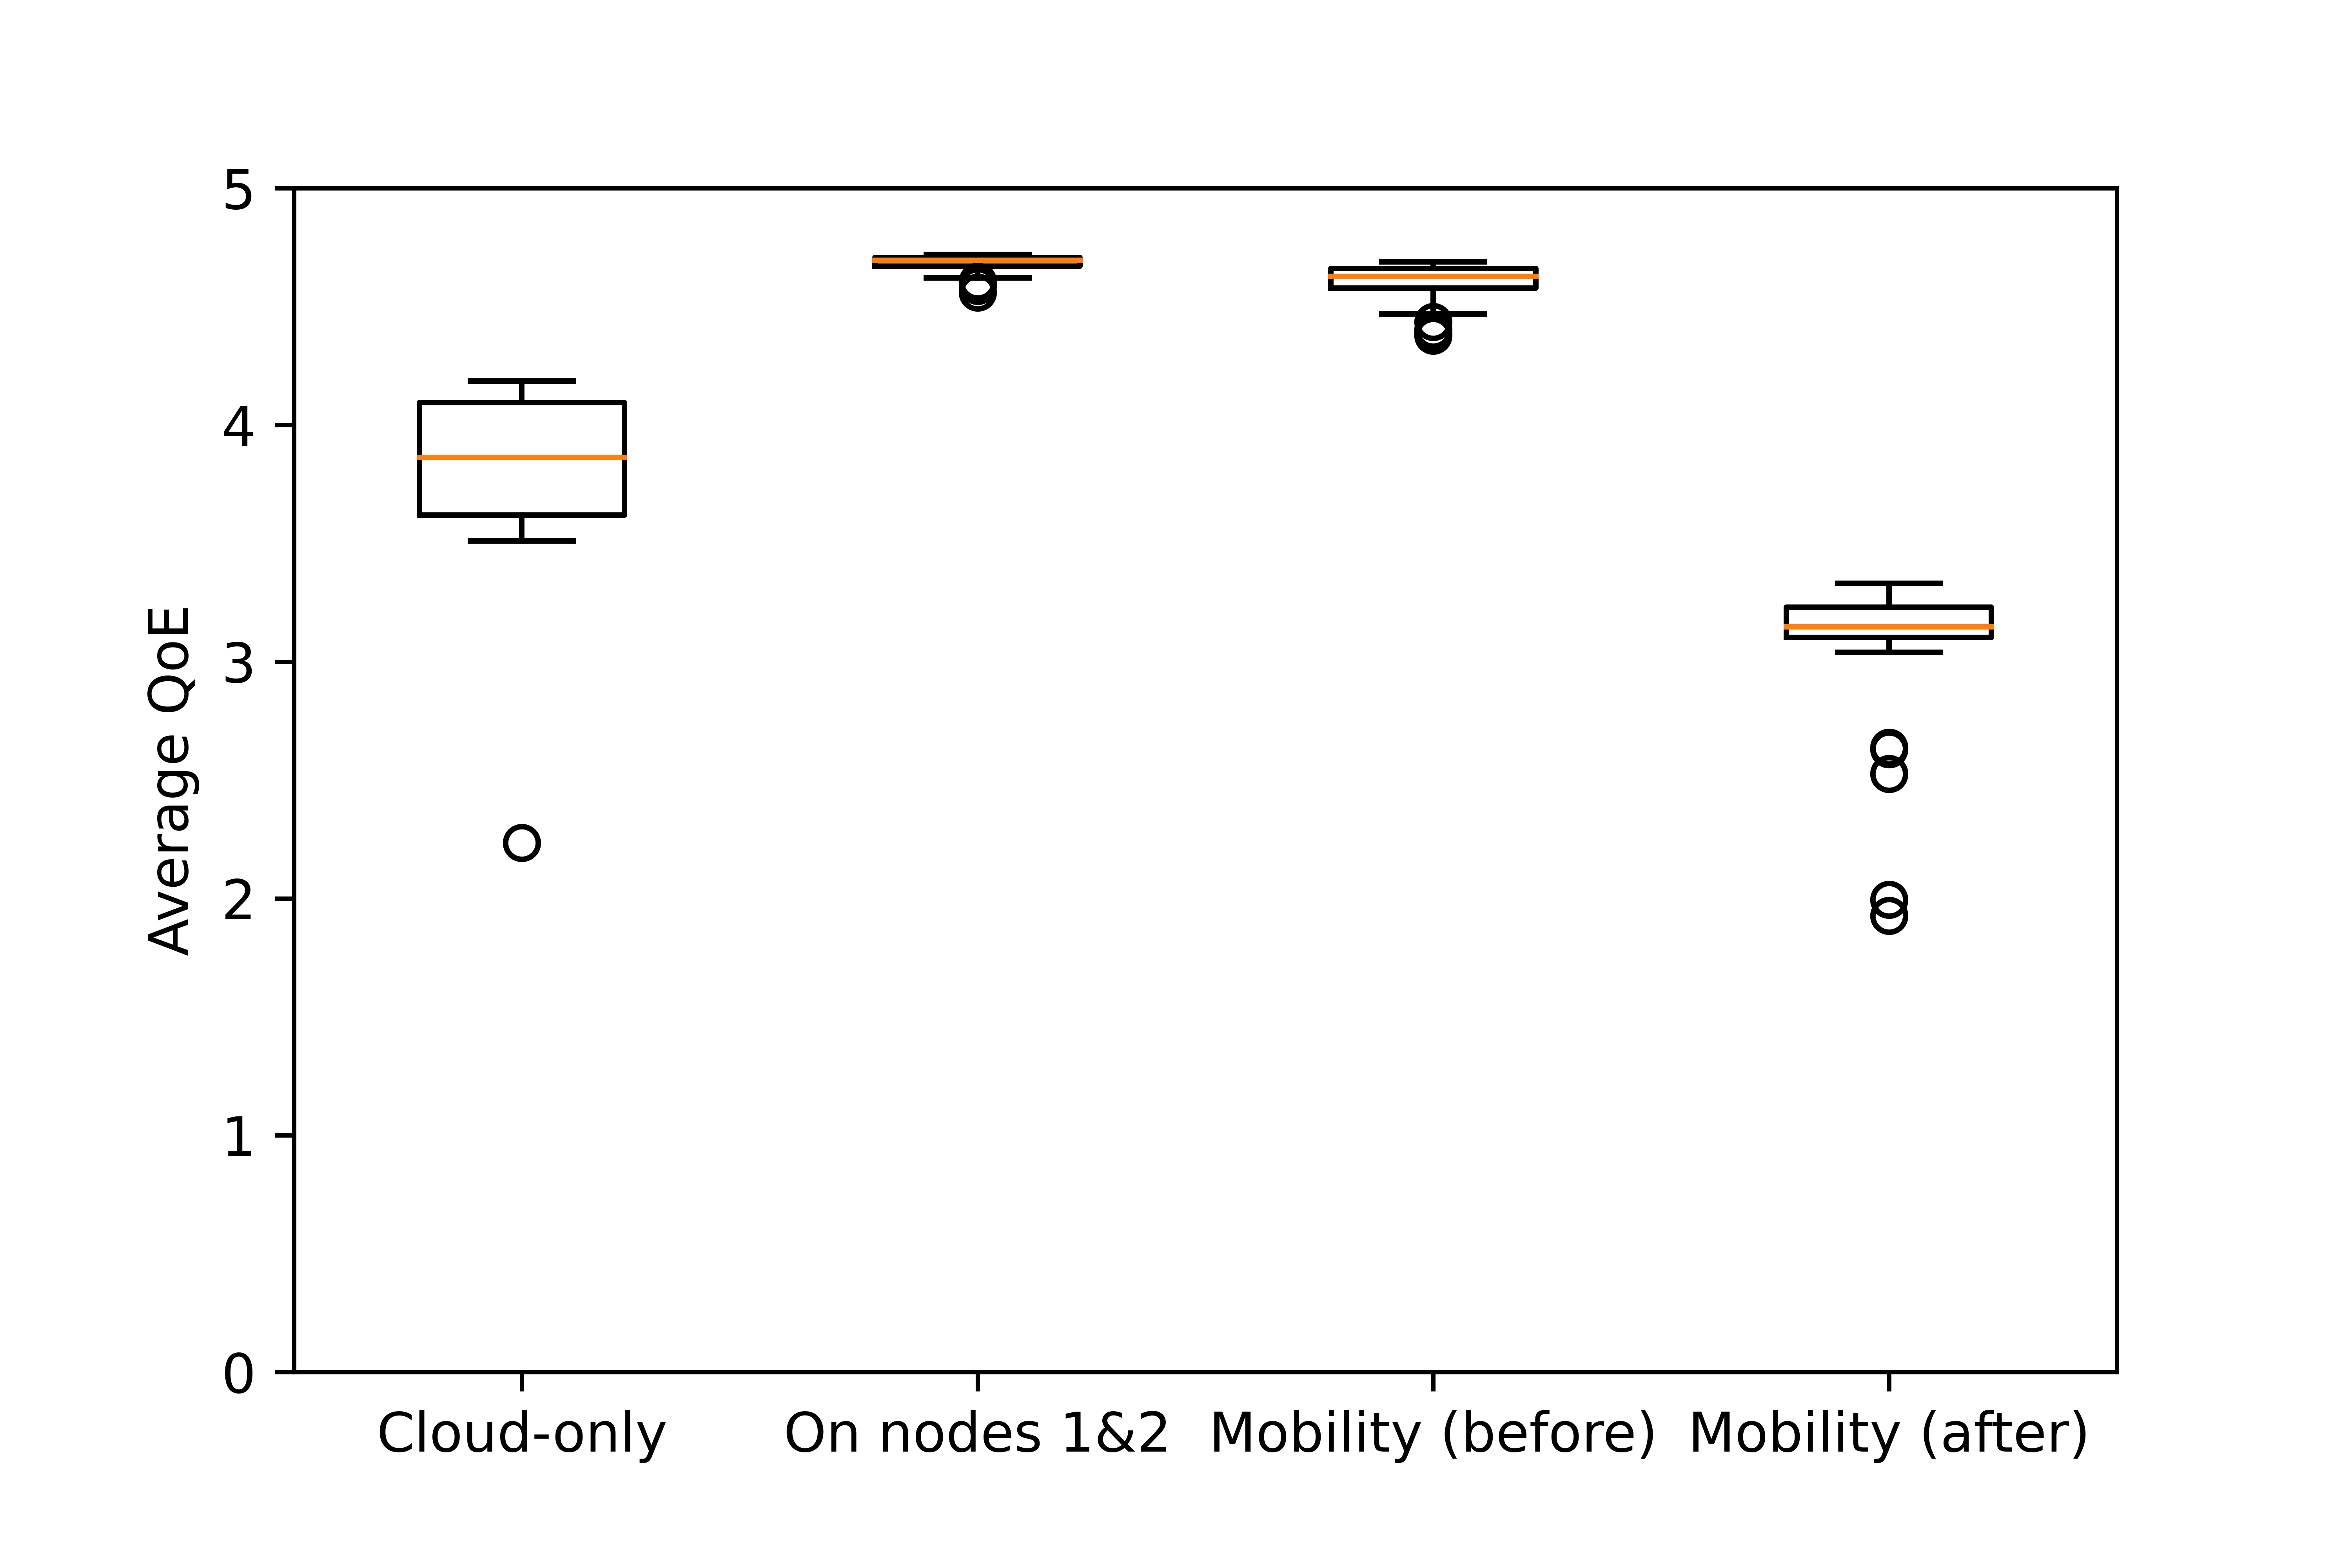
\includegraphics[width=0.31\linewidth]{images/QoEBoxplot-15u.png}
    \label{fig:red-comparison-plot}
    }
    \subfigure[]{
    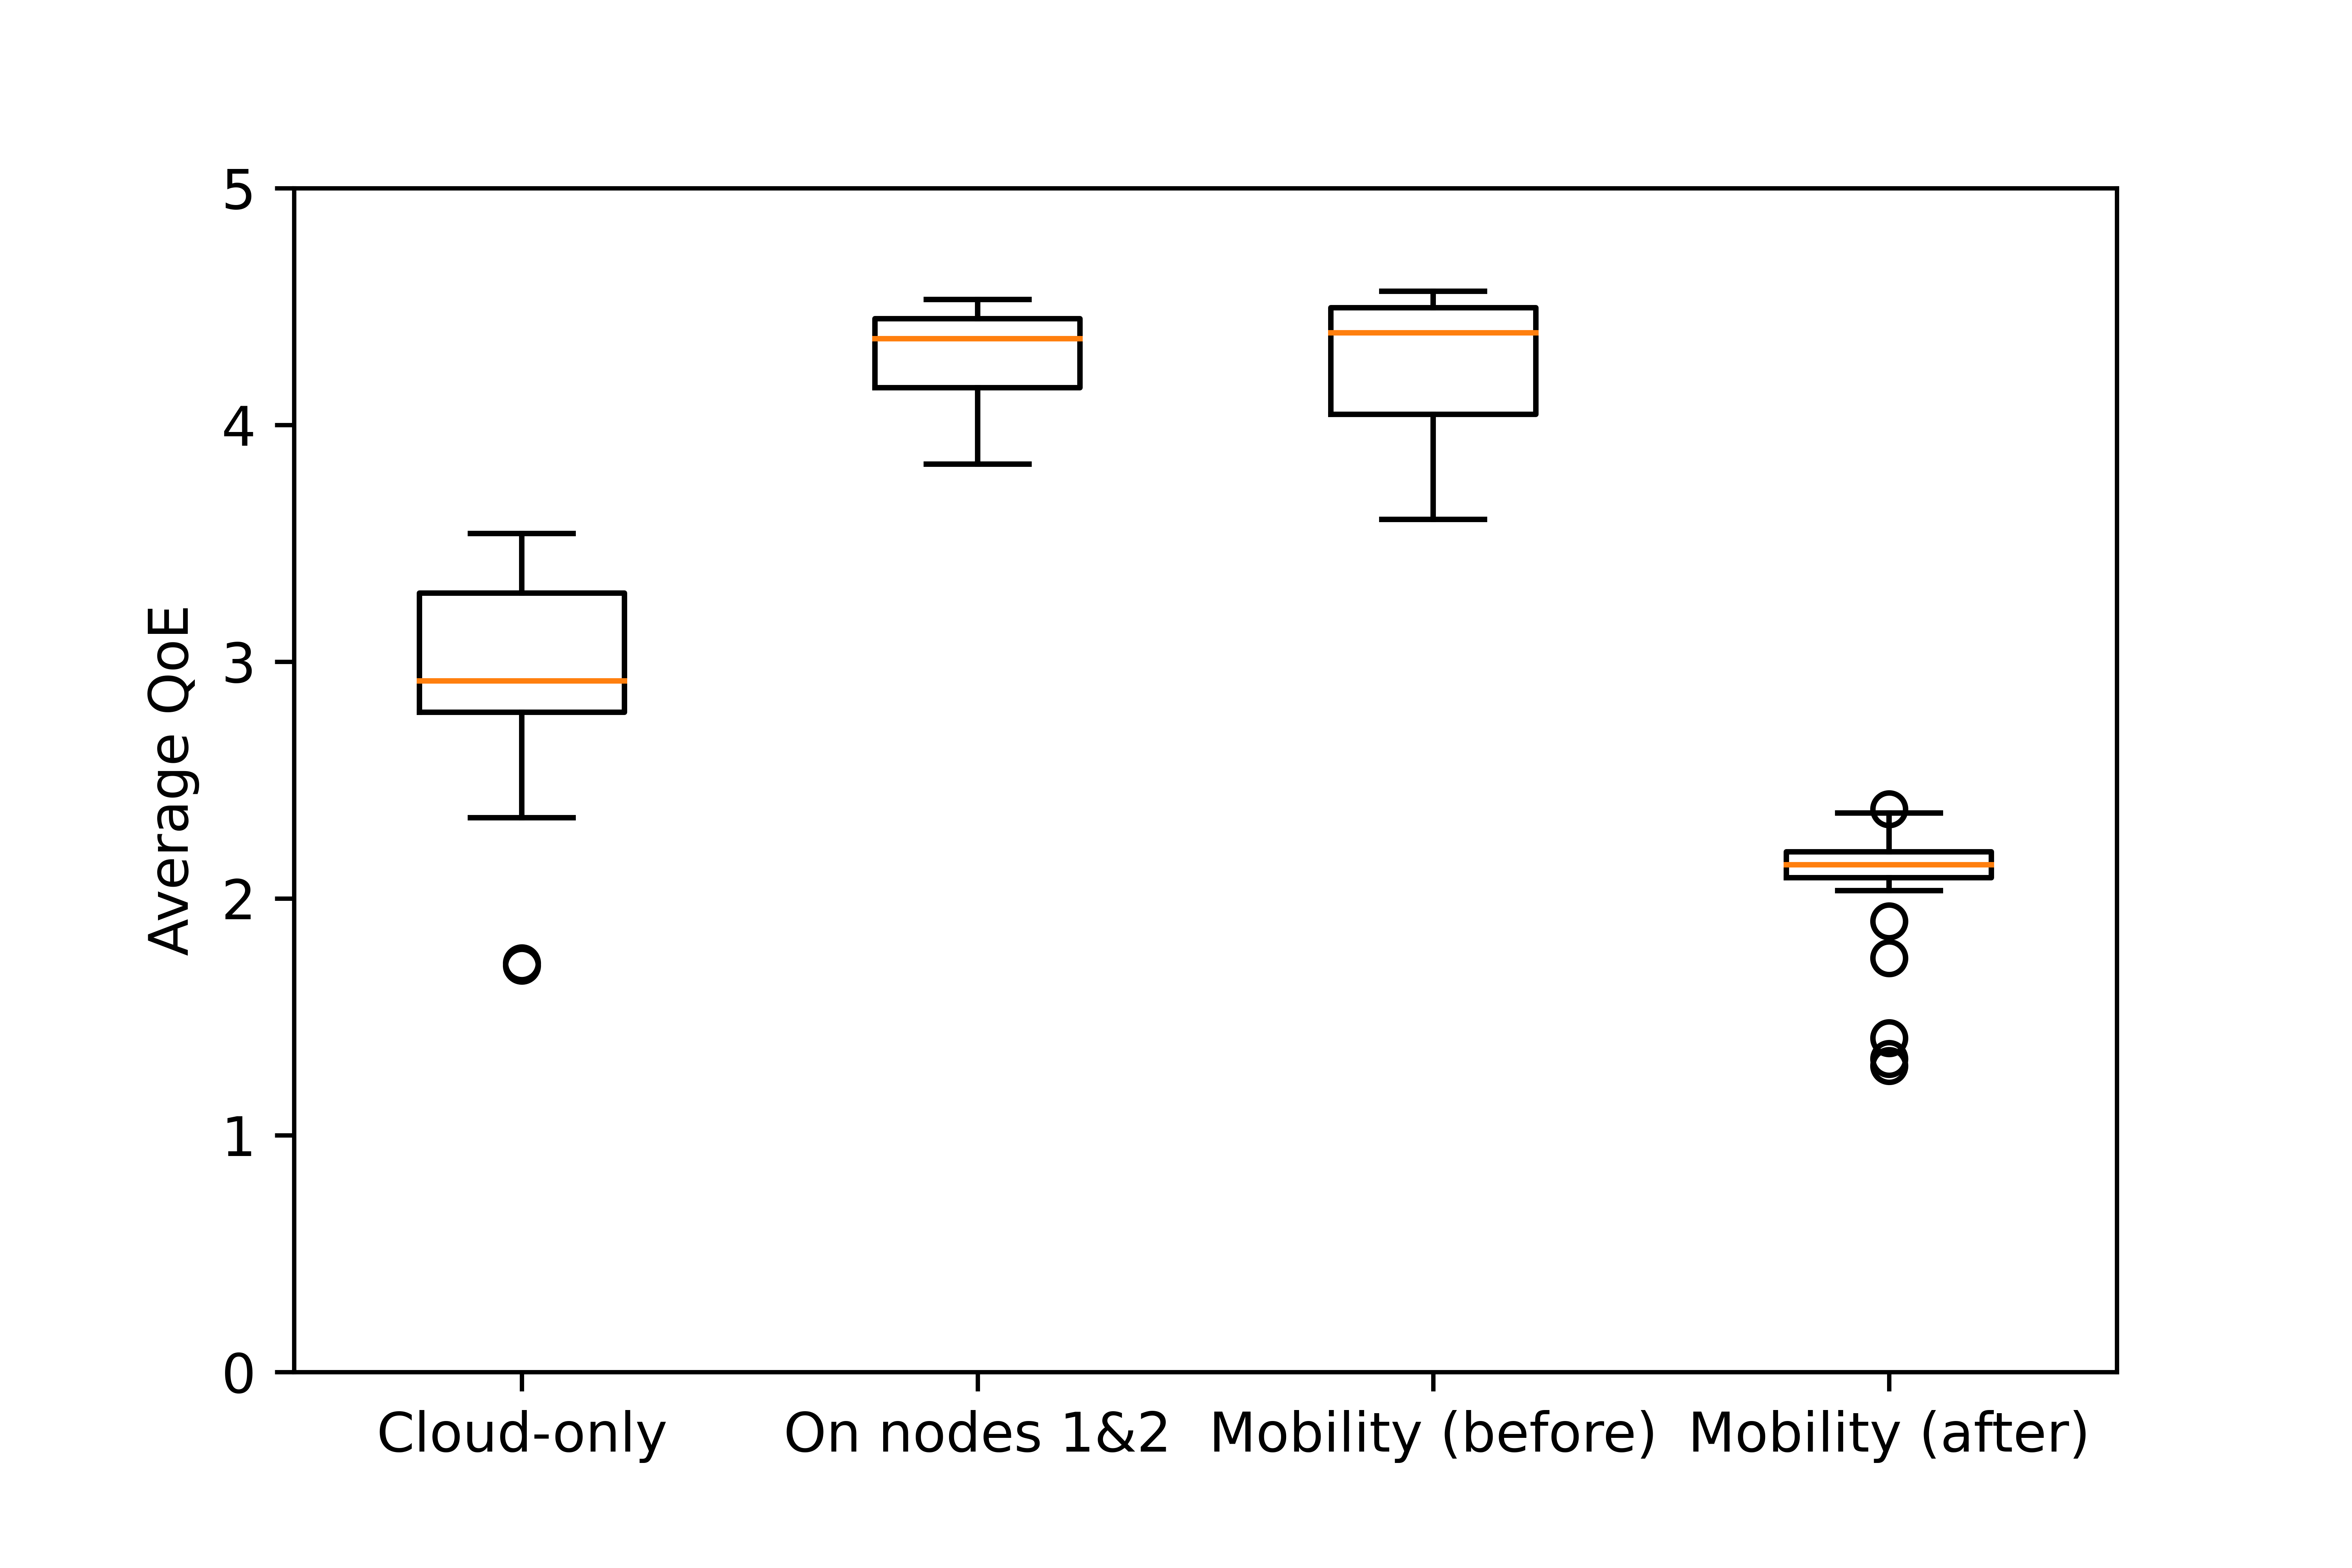
\includegraphics[width=0.31\linewidth]{images/QoEBoxplot-20u.png}
    \label{fig:co-comparison-boxplot}
    }
    \subfigure[]{
    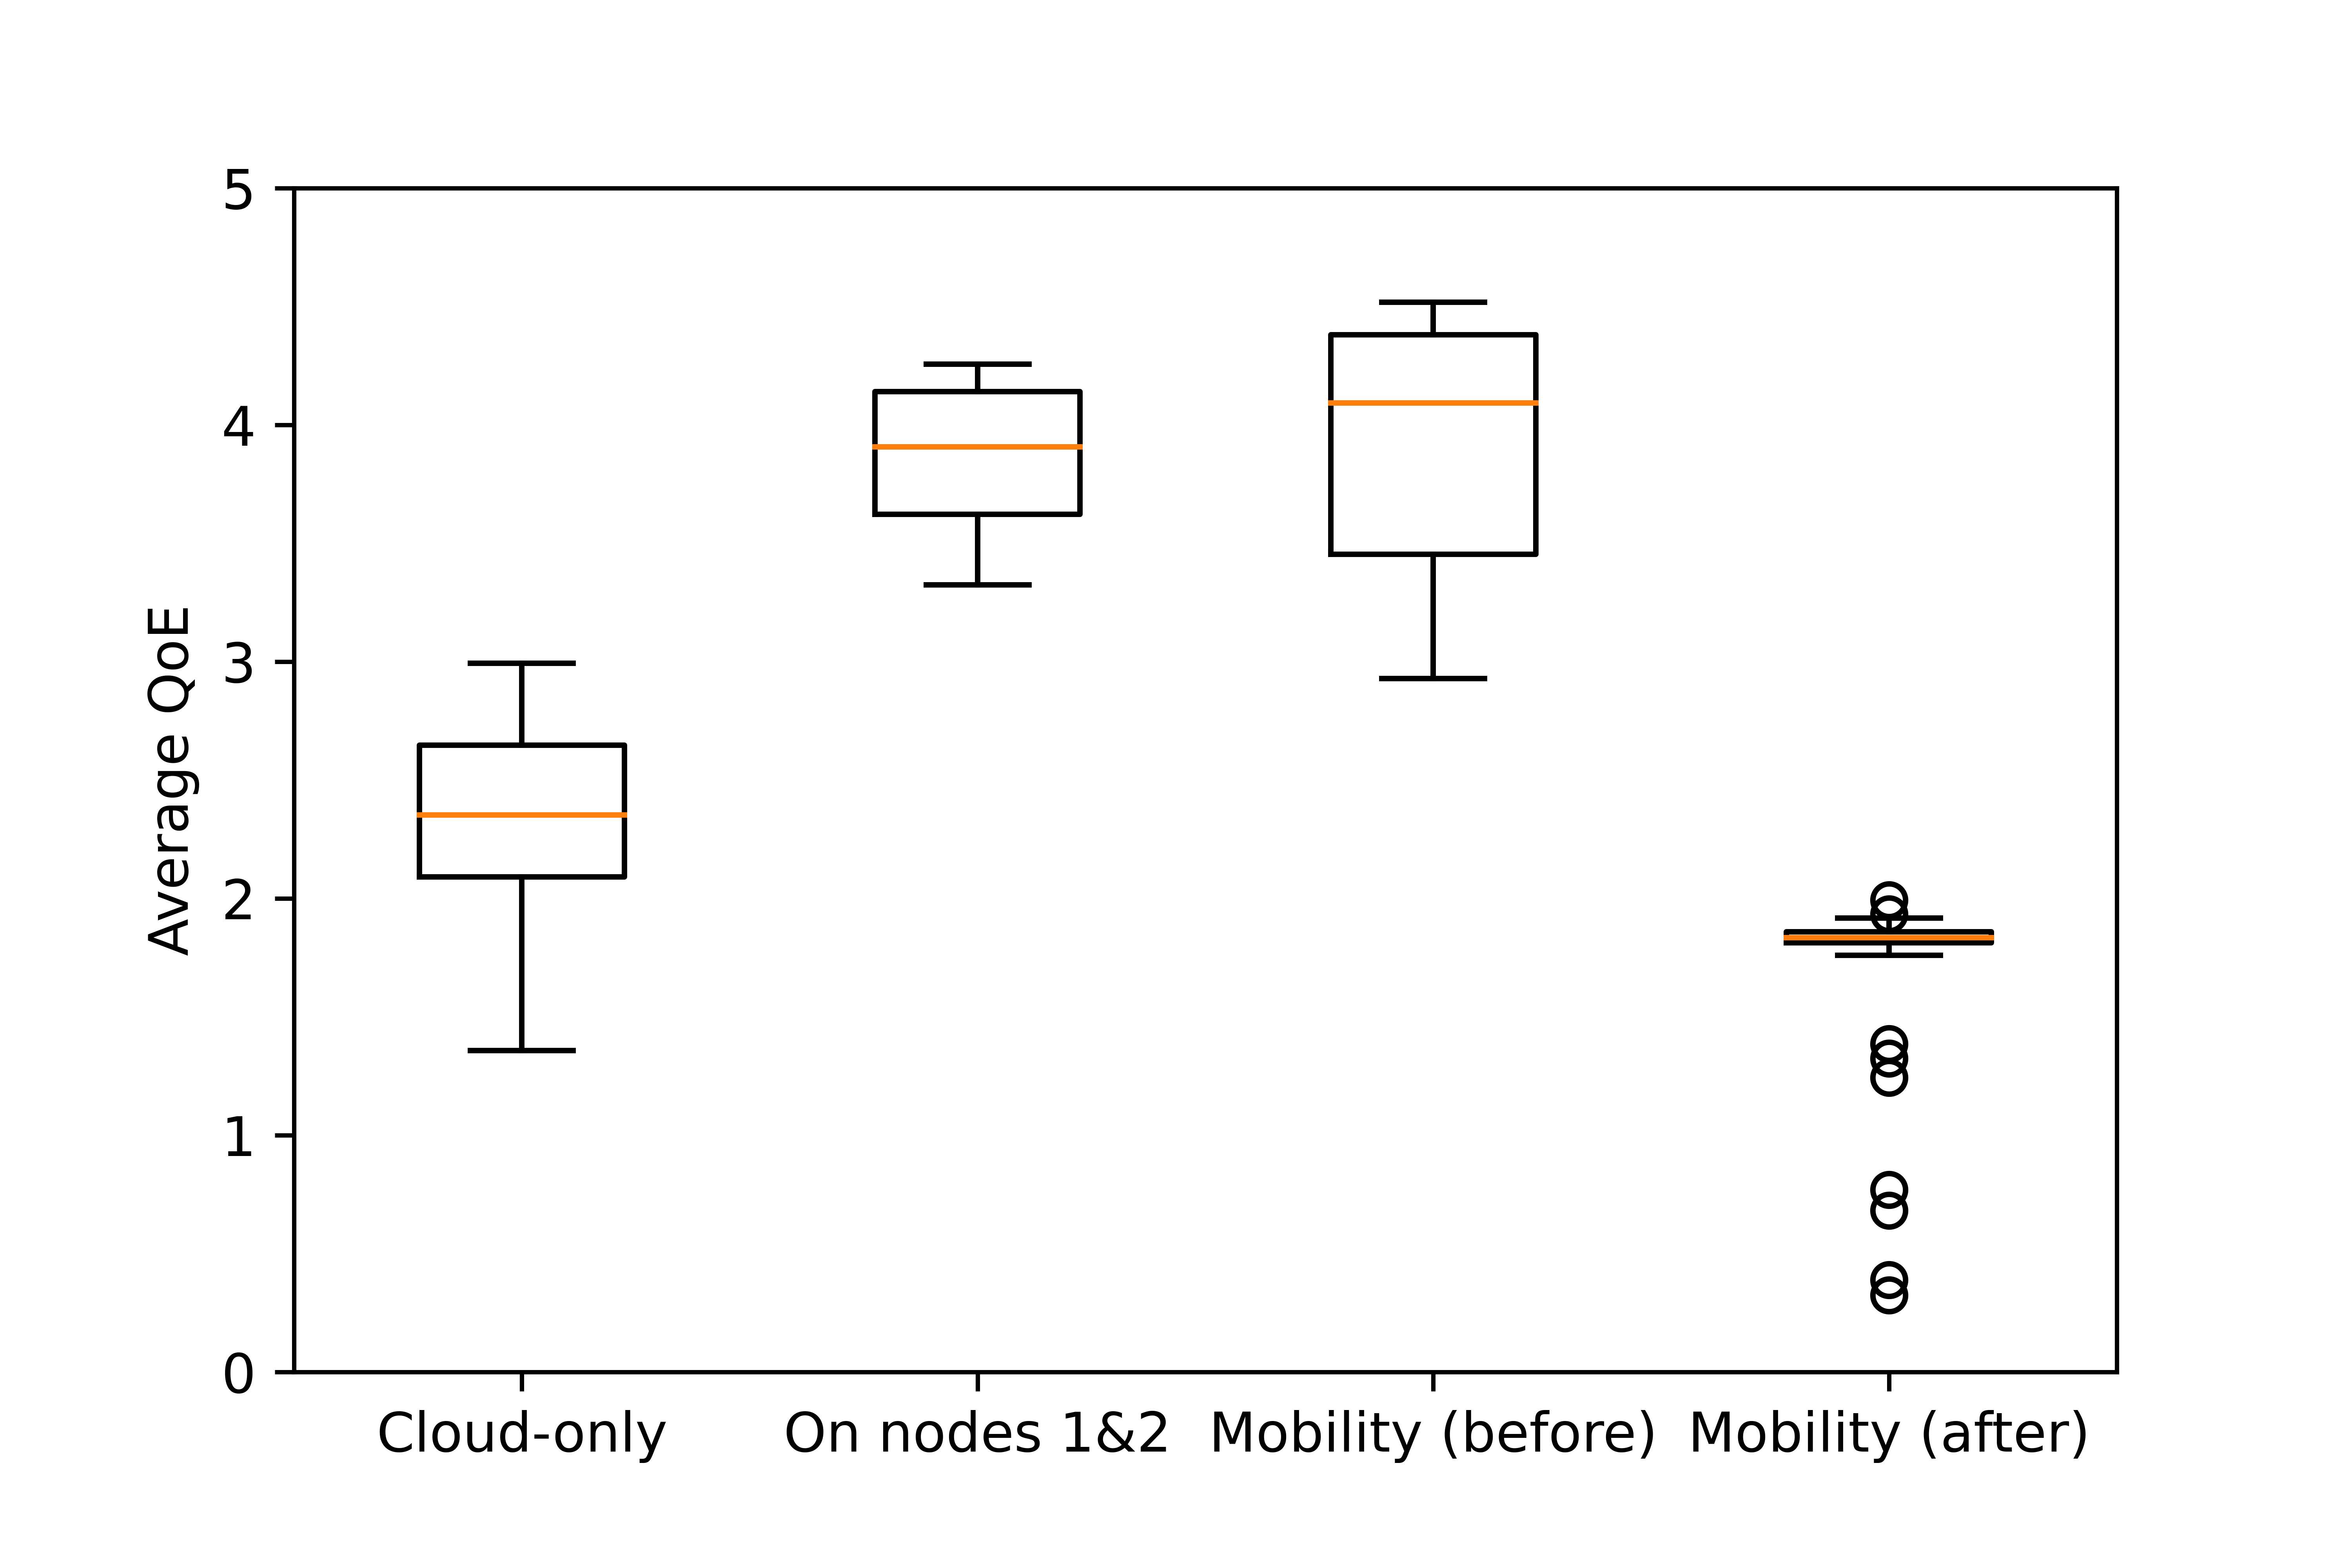
\includegraphics[width=0.31\linewidth]{images/QoEBoxplot-25u.png}
    \label{fig:red-comparison-plot}
    }
    
    \caption{Average QoE results for scenarios with 15, 20 and 25 users per AP.}
    \label{fig:comparison-rof-2}
\end{figure*}


\begin{figure*}
    \centering
    \subfigure[]{
    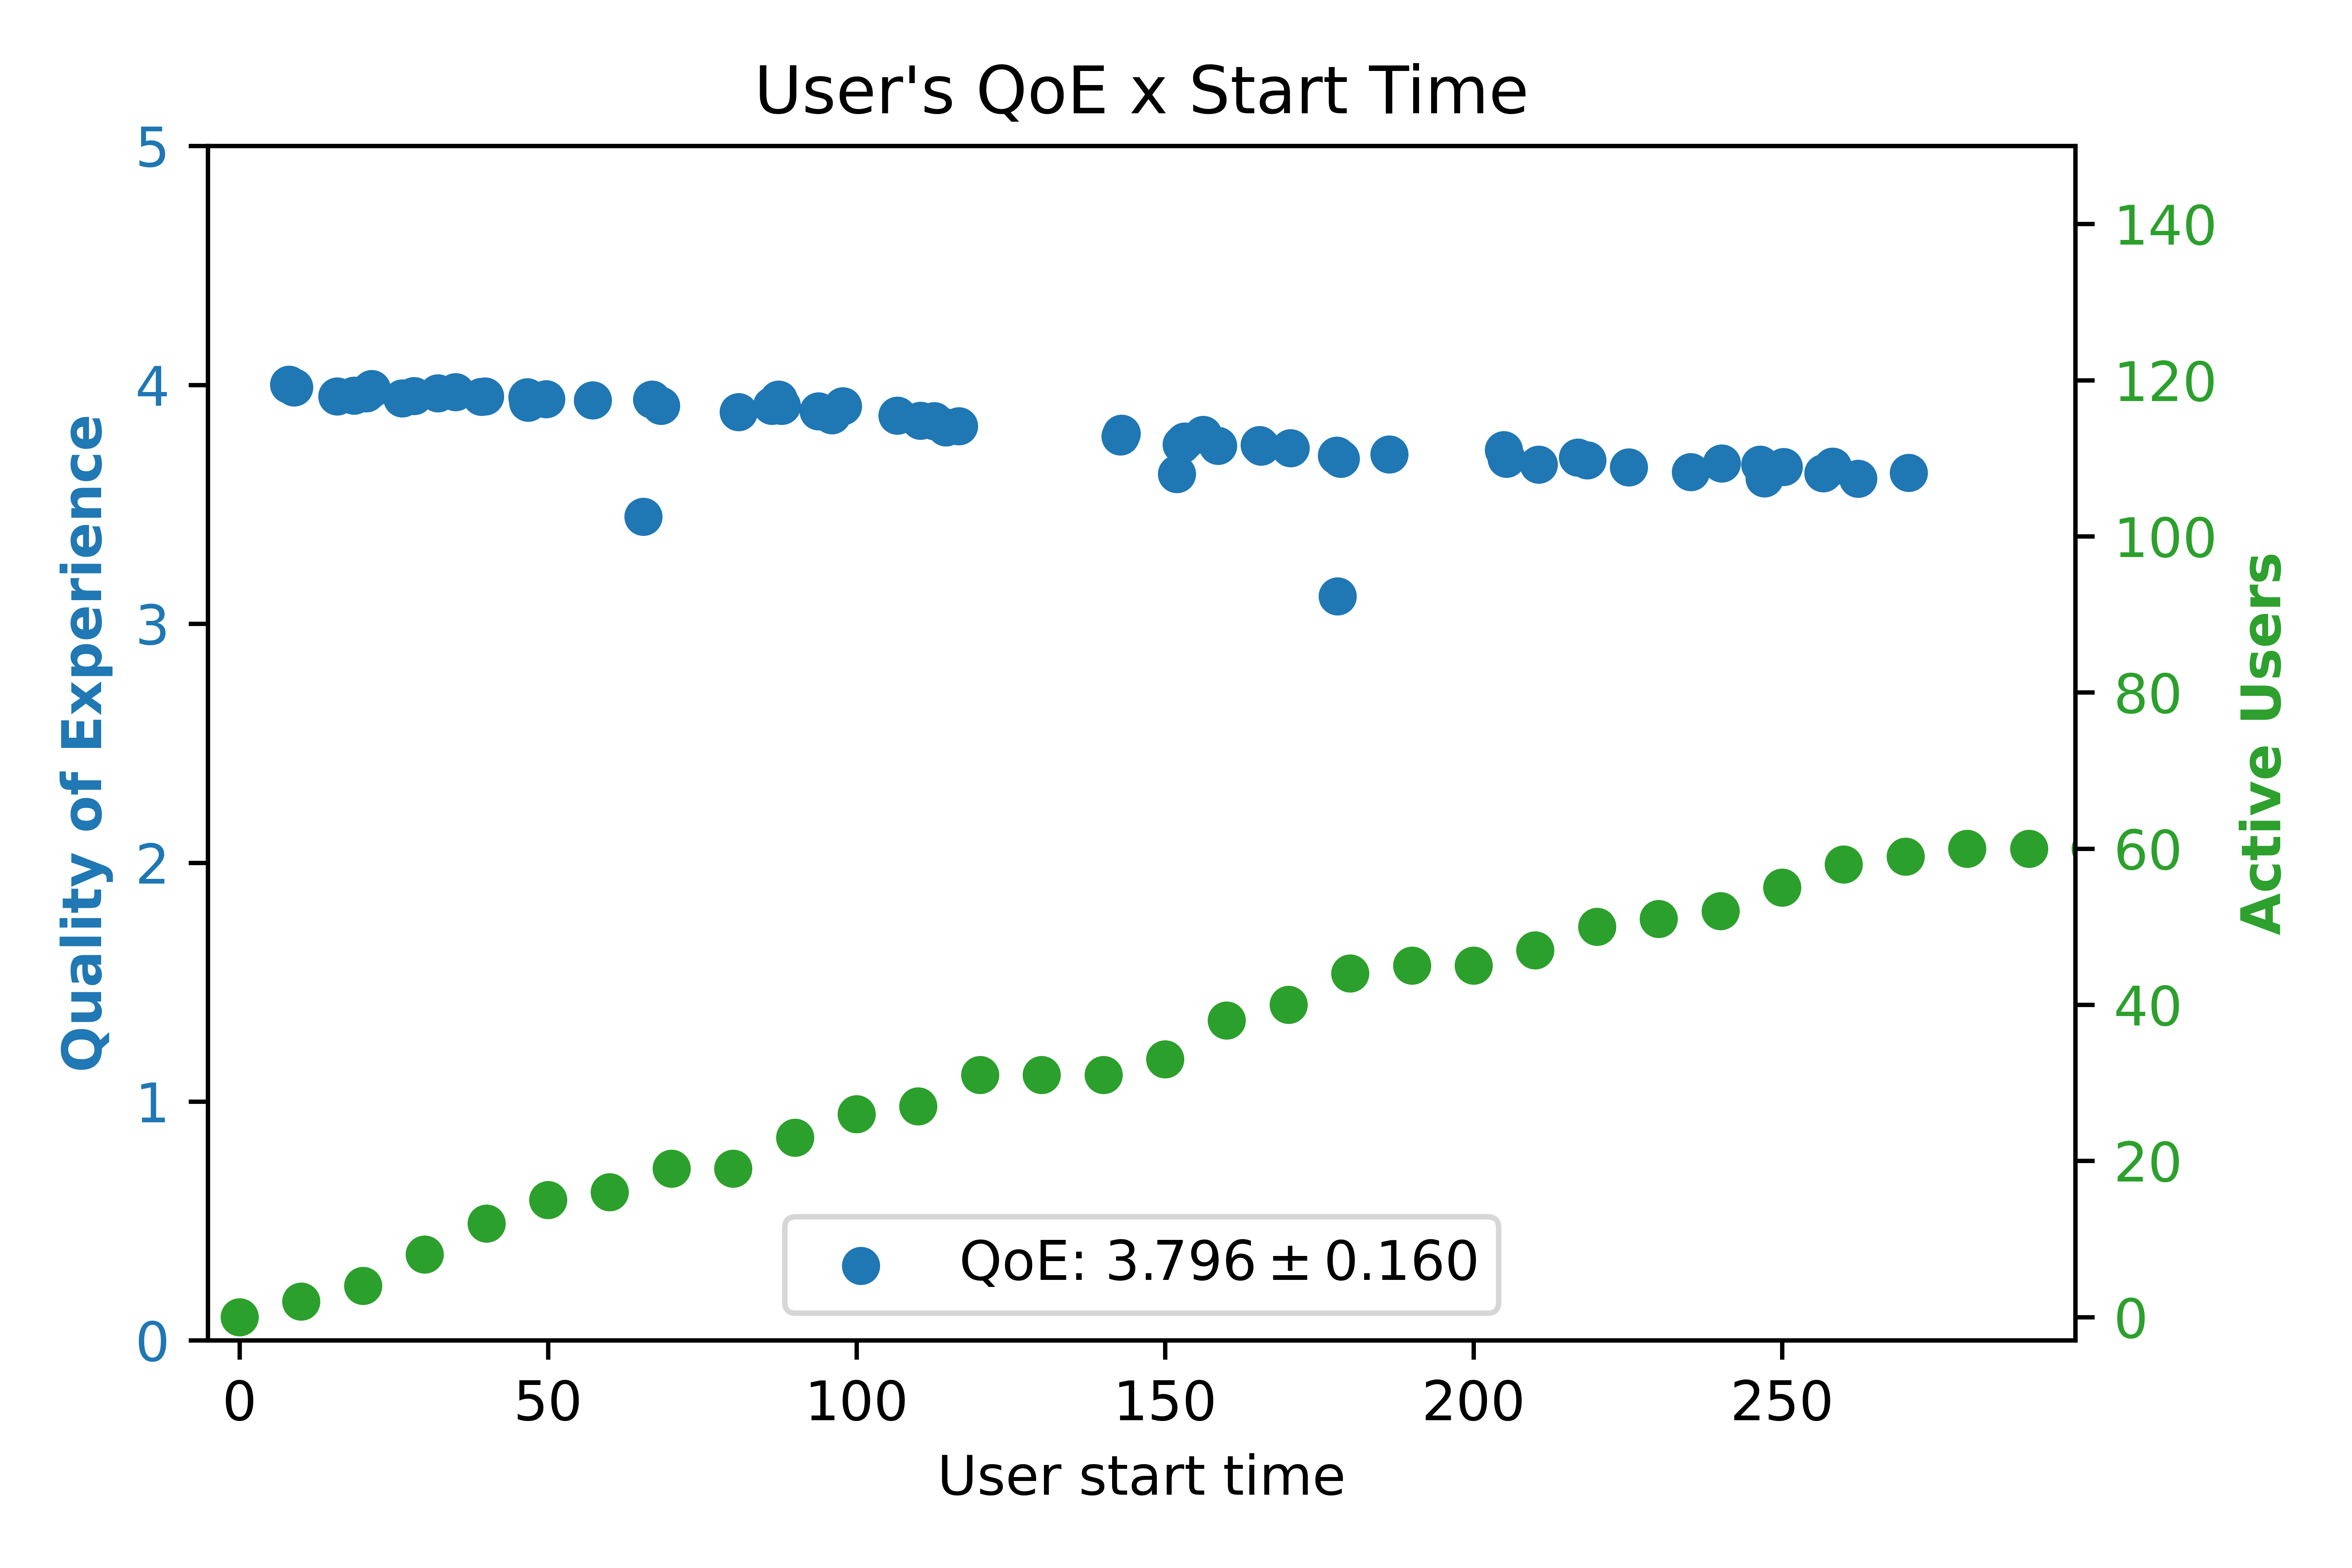
\includegraphics[width=0.31\linewidth]{images/cloud_QoExStartTime15.png}
    \label{fig:rssi-comparison-2}
    }
    \subfigure[]{
    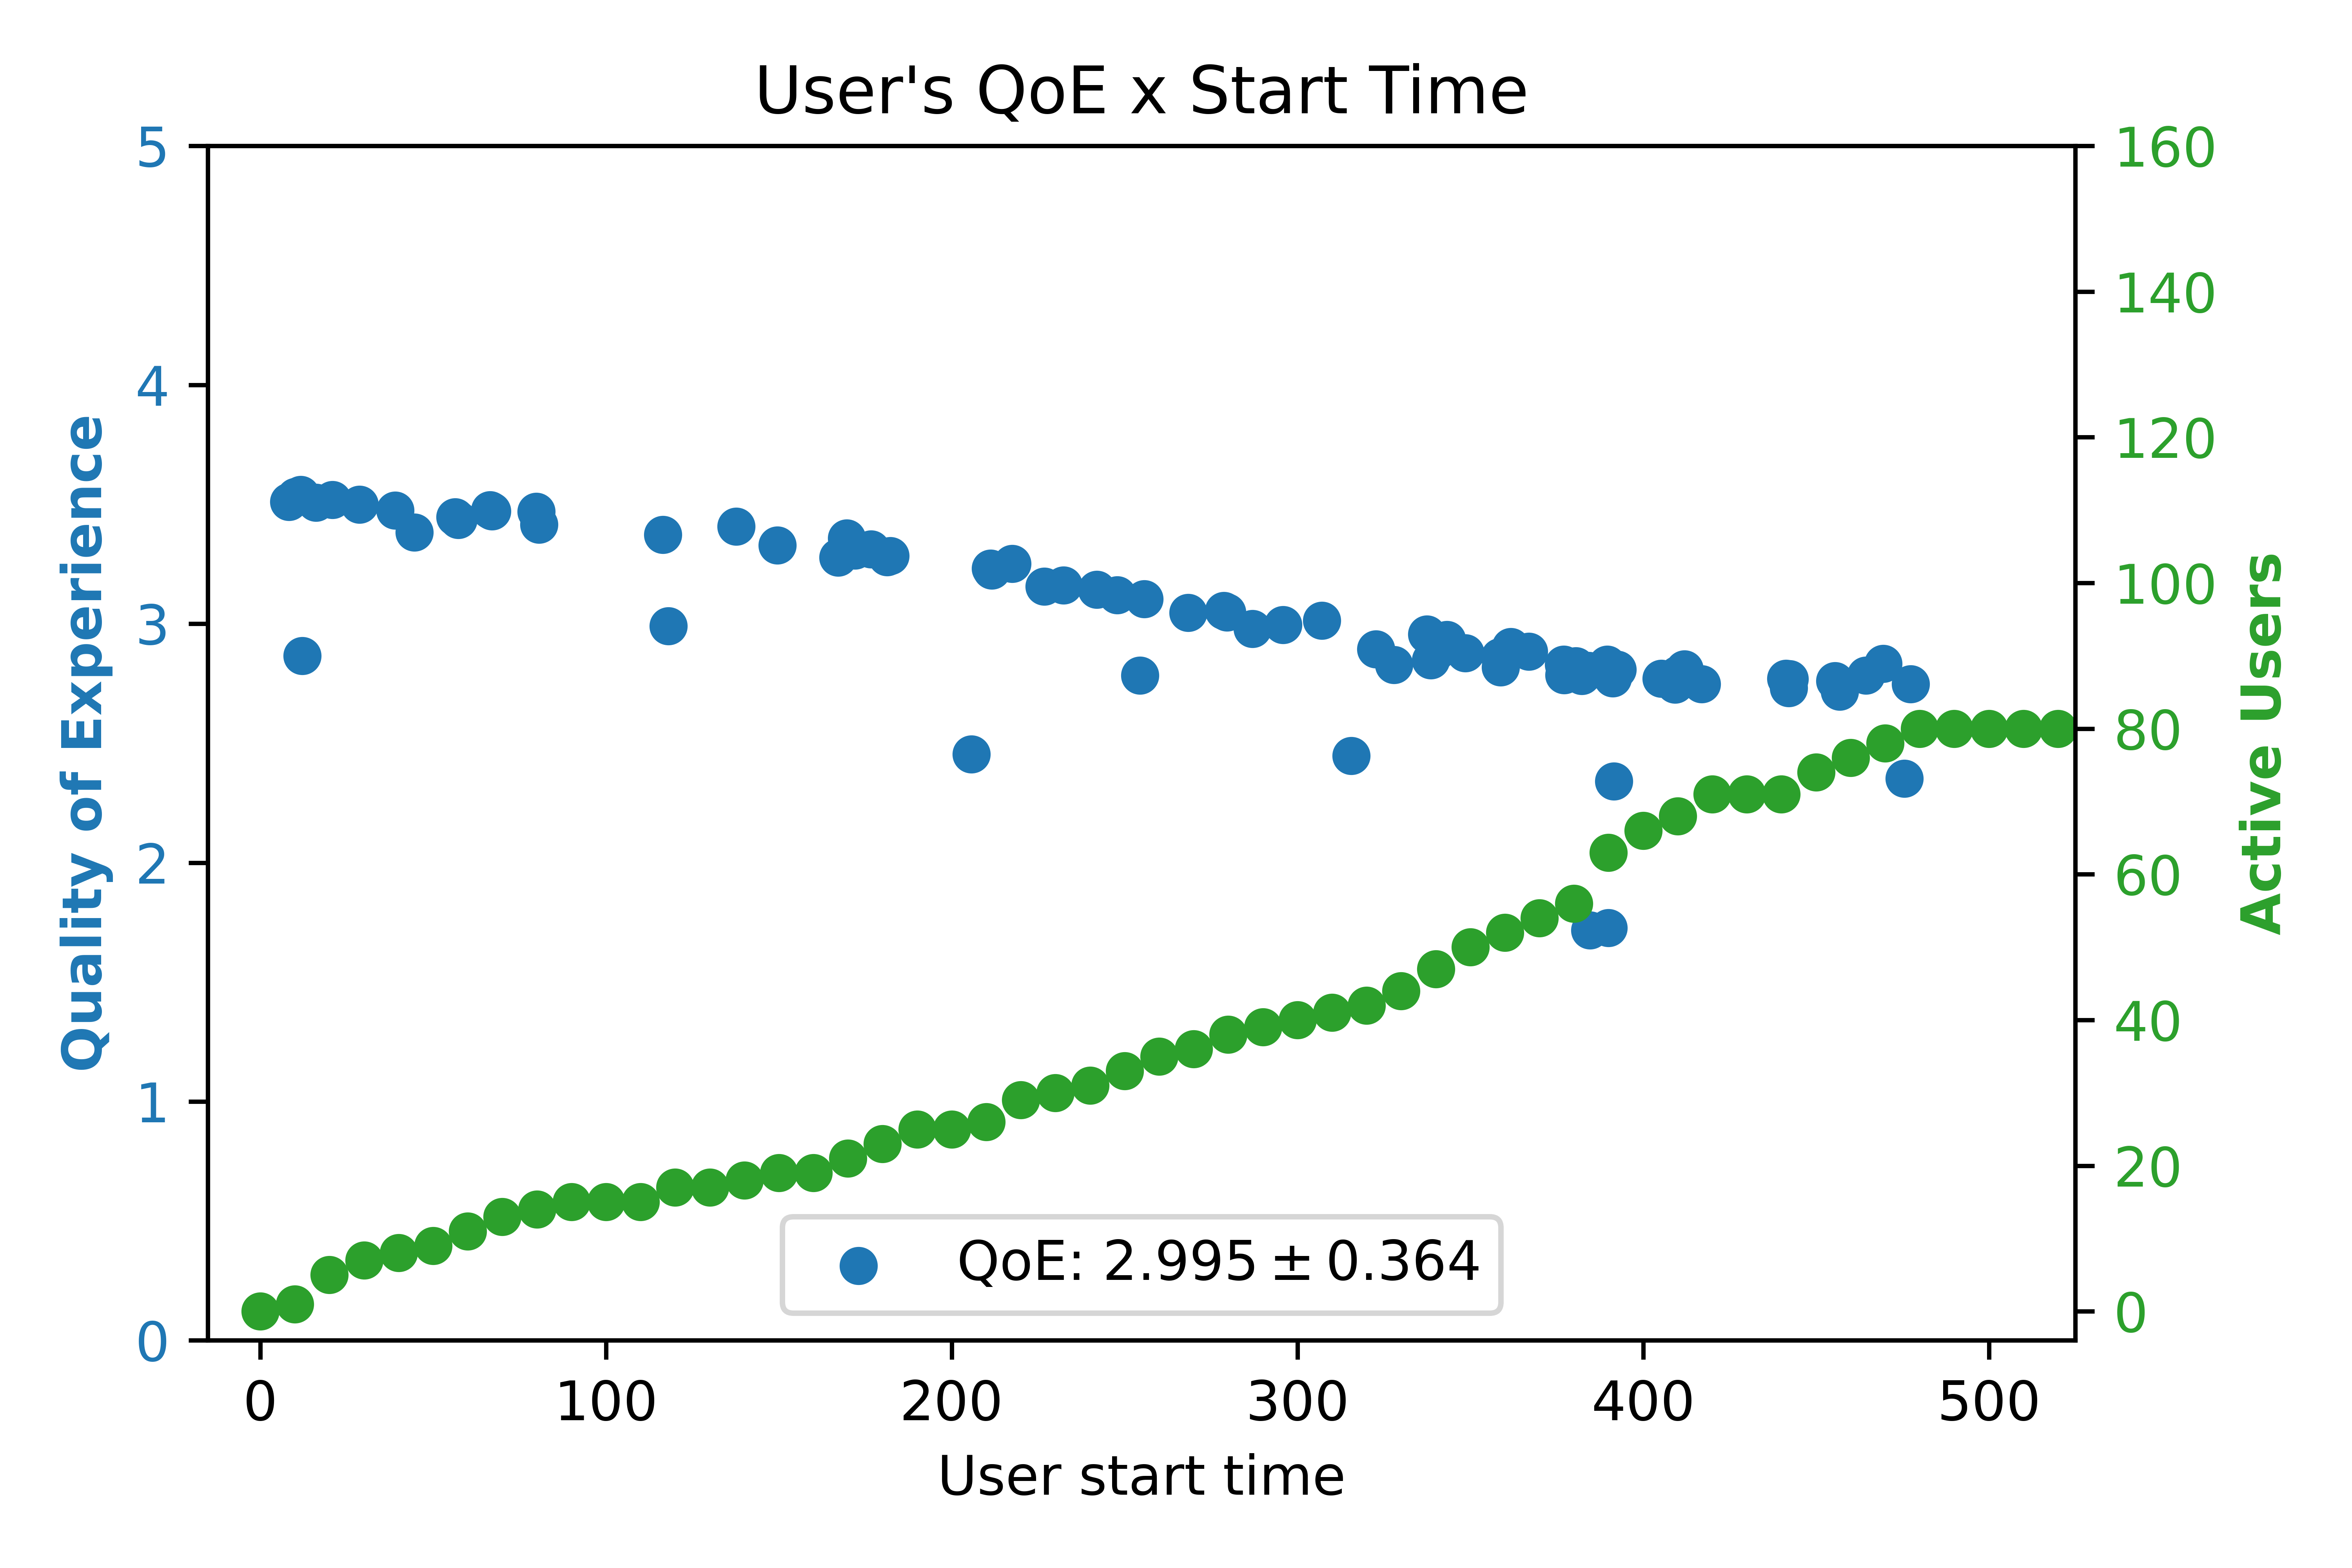
\includegraphics[width=0.31\linewidth]{images/cloud_QoExStartTime20.png}
    \label{fig:plr-comparison-2}
    }
    \subfigure[]{
    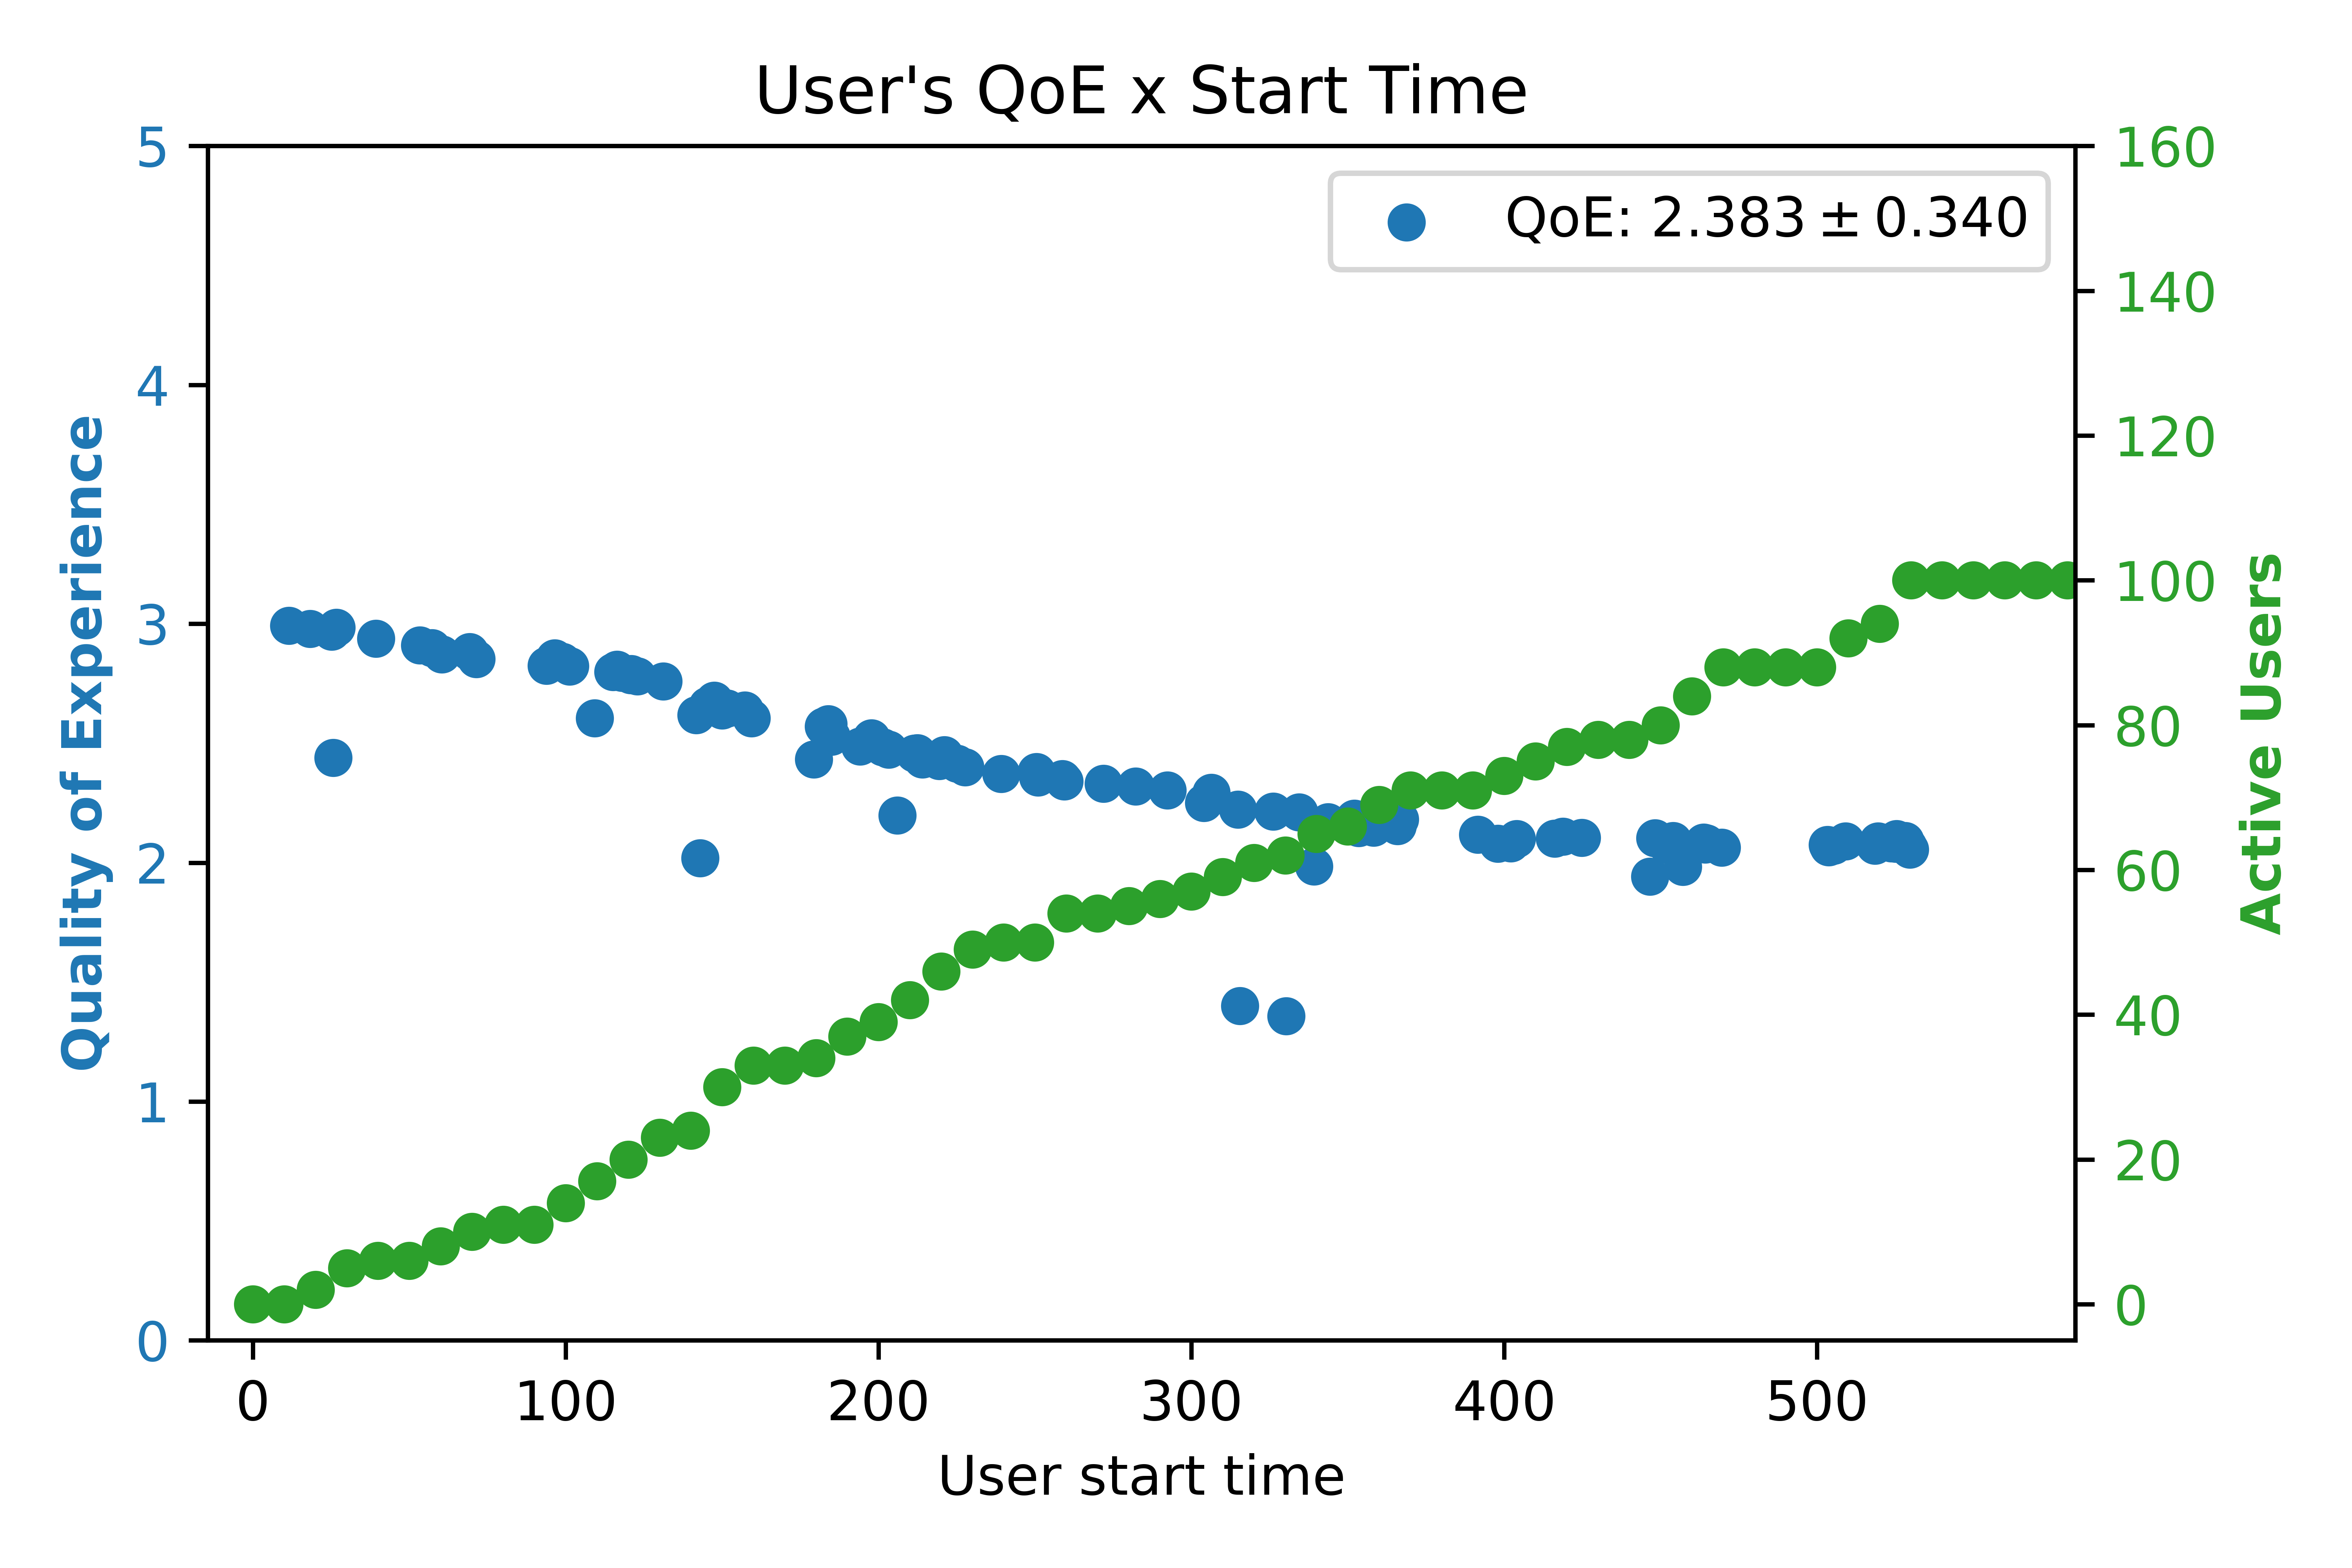
\includegraphics[width=0.31\linewidth]{images/cloud_QoExStartTime25.png}
    \label{fig:plr-comparison-2}
    }
    
    \subfigure[]{
    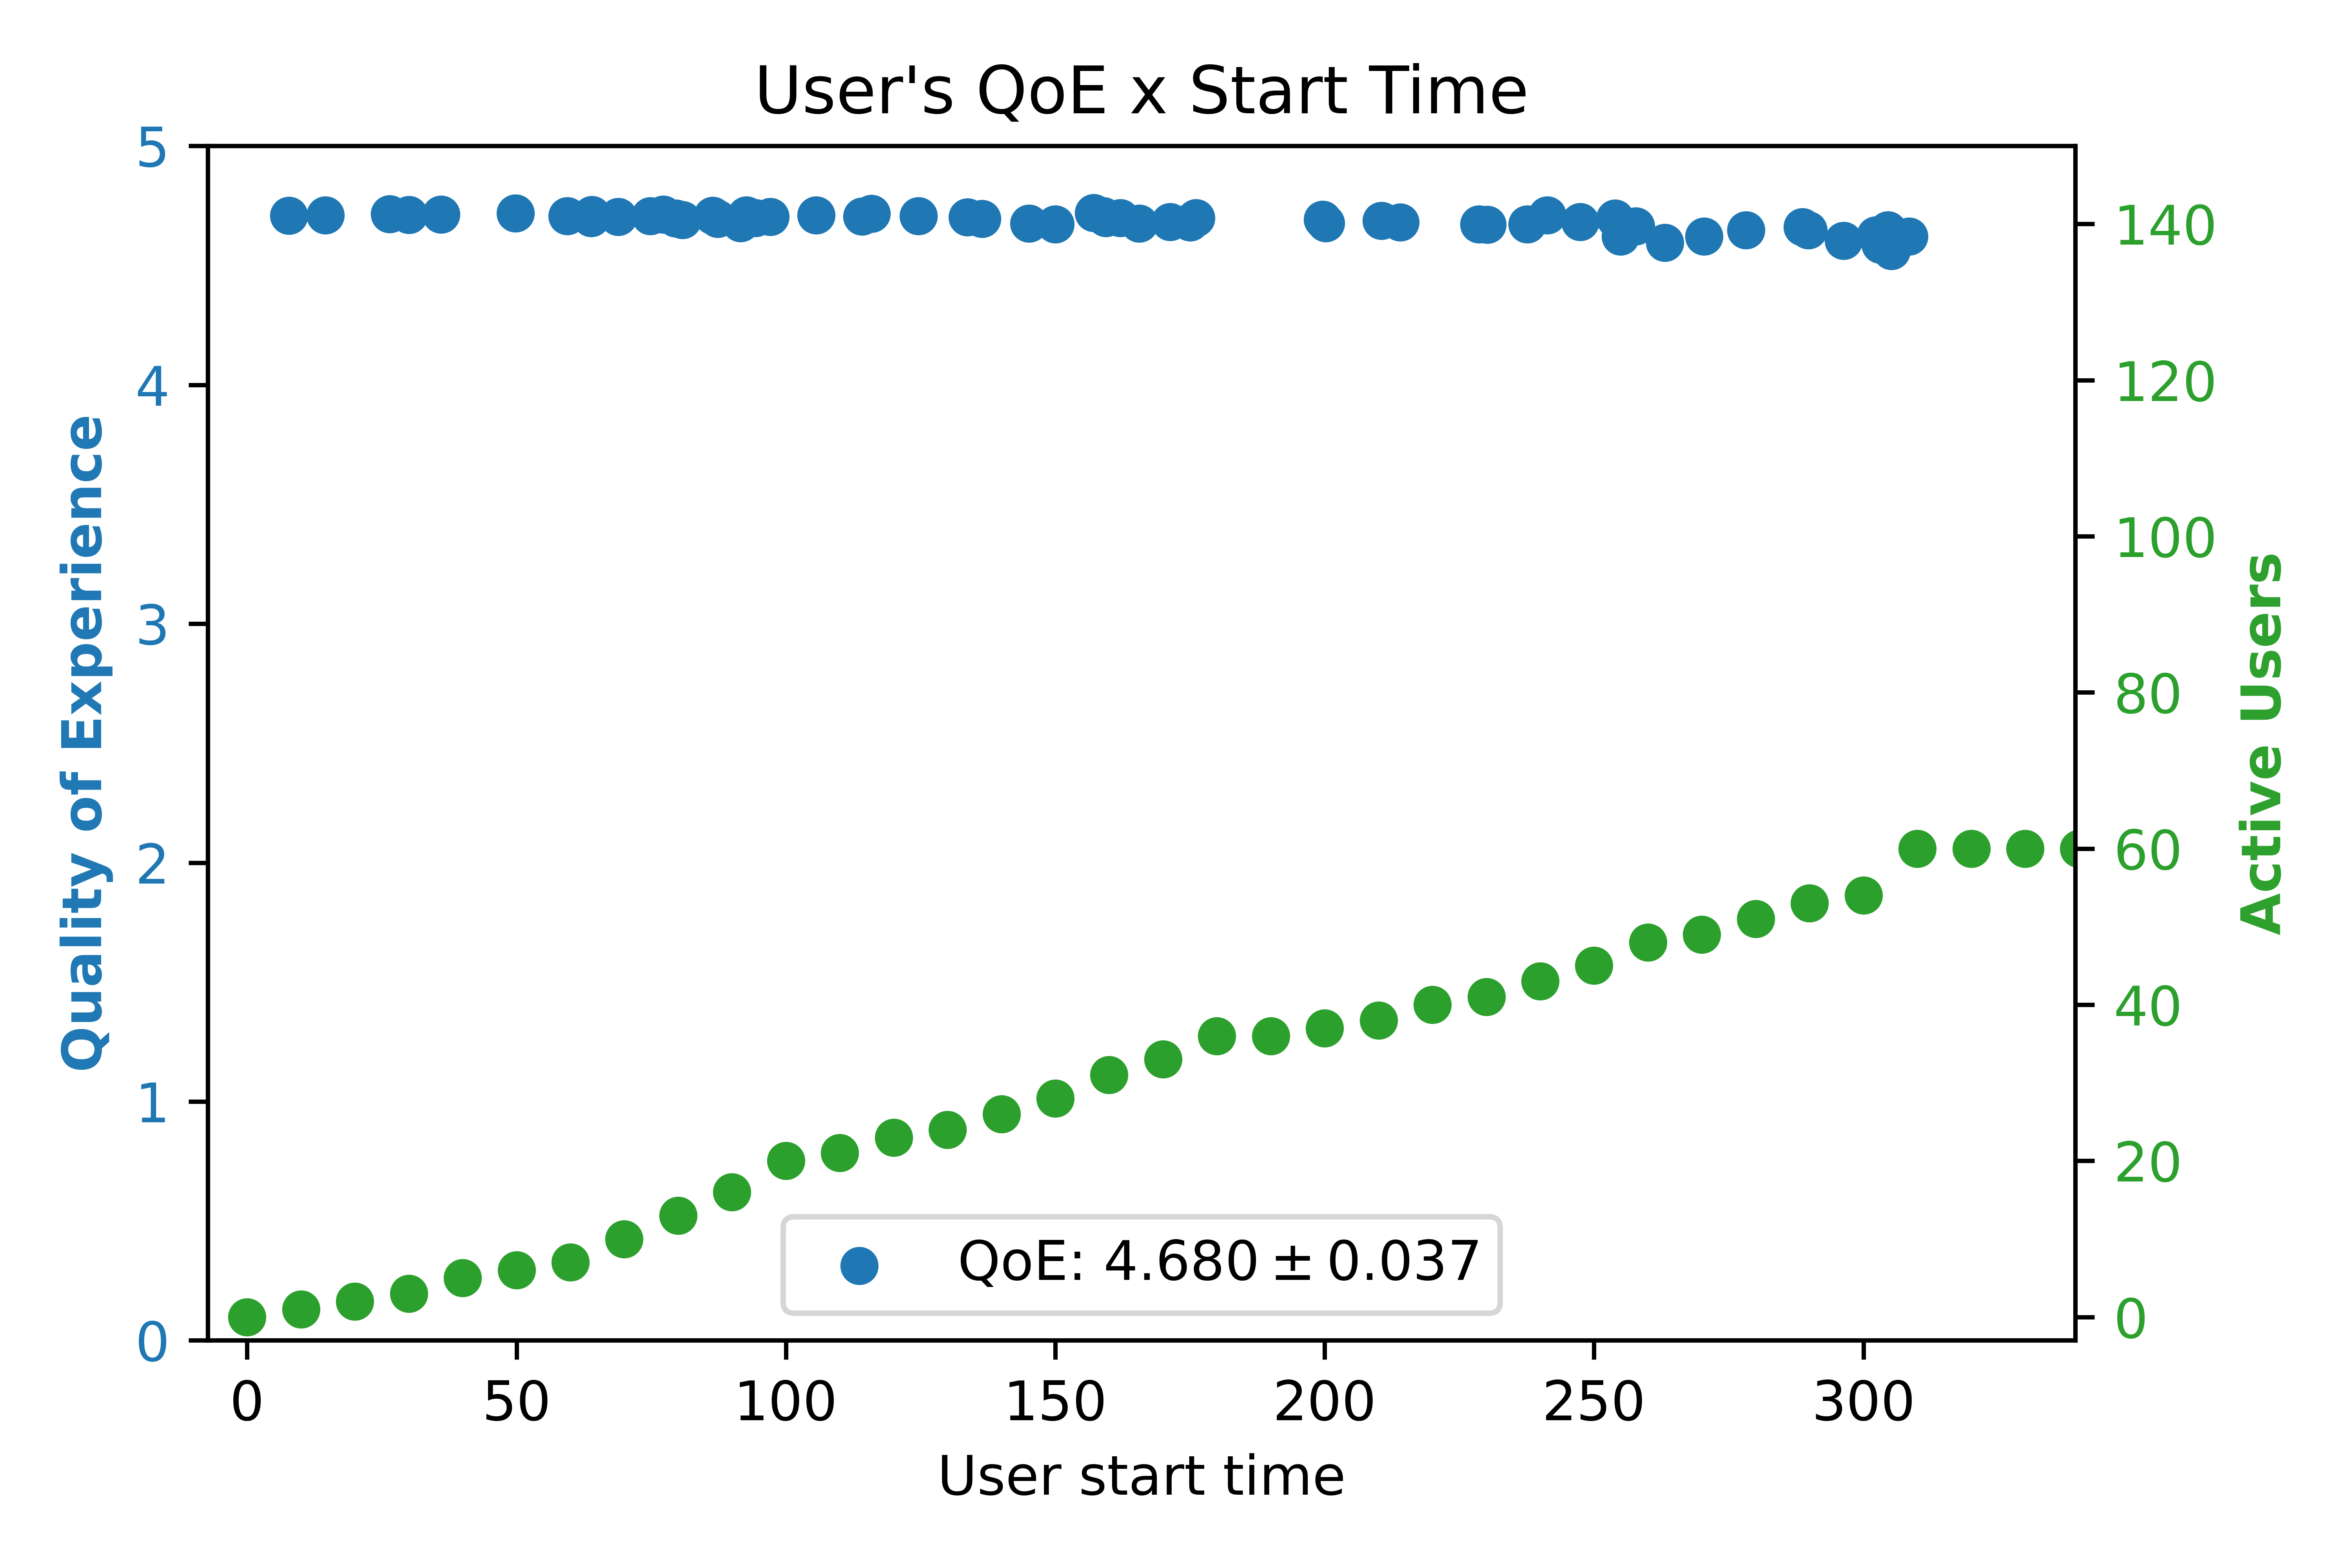
\includegraphics[width=0.31\linewidth]{images/Redicrect_QoExStartTime15.png}
    \label{fig:rssi-comparison-2}
    }
    \subfigure[]{
    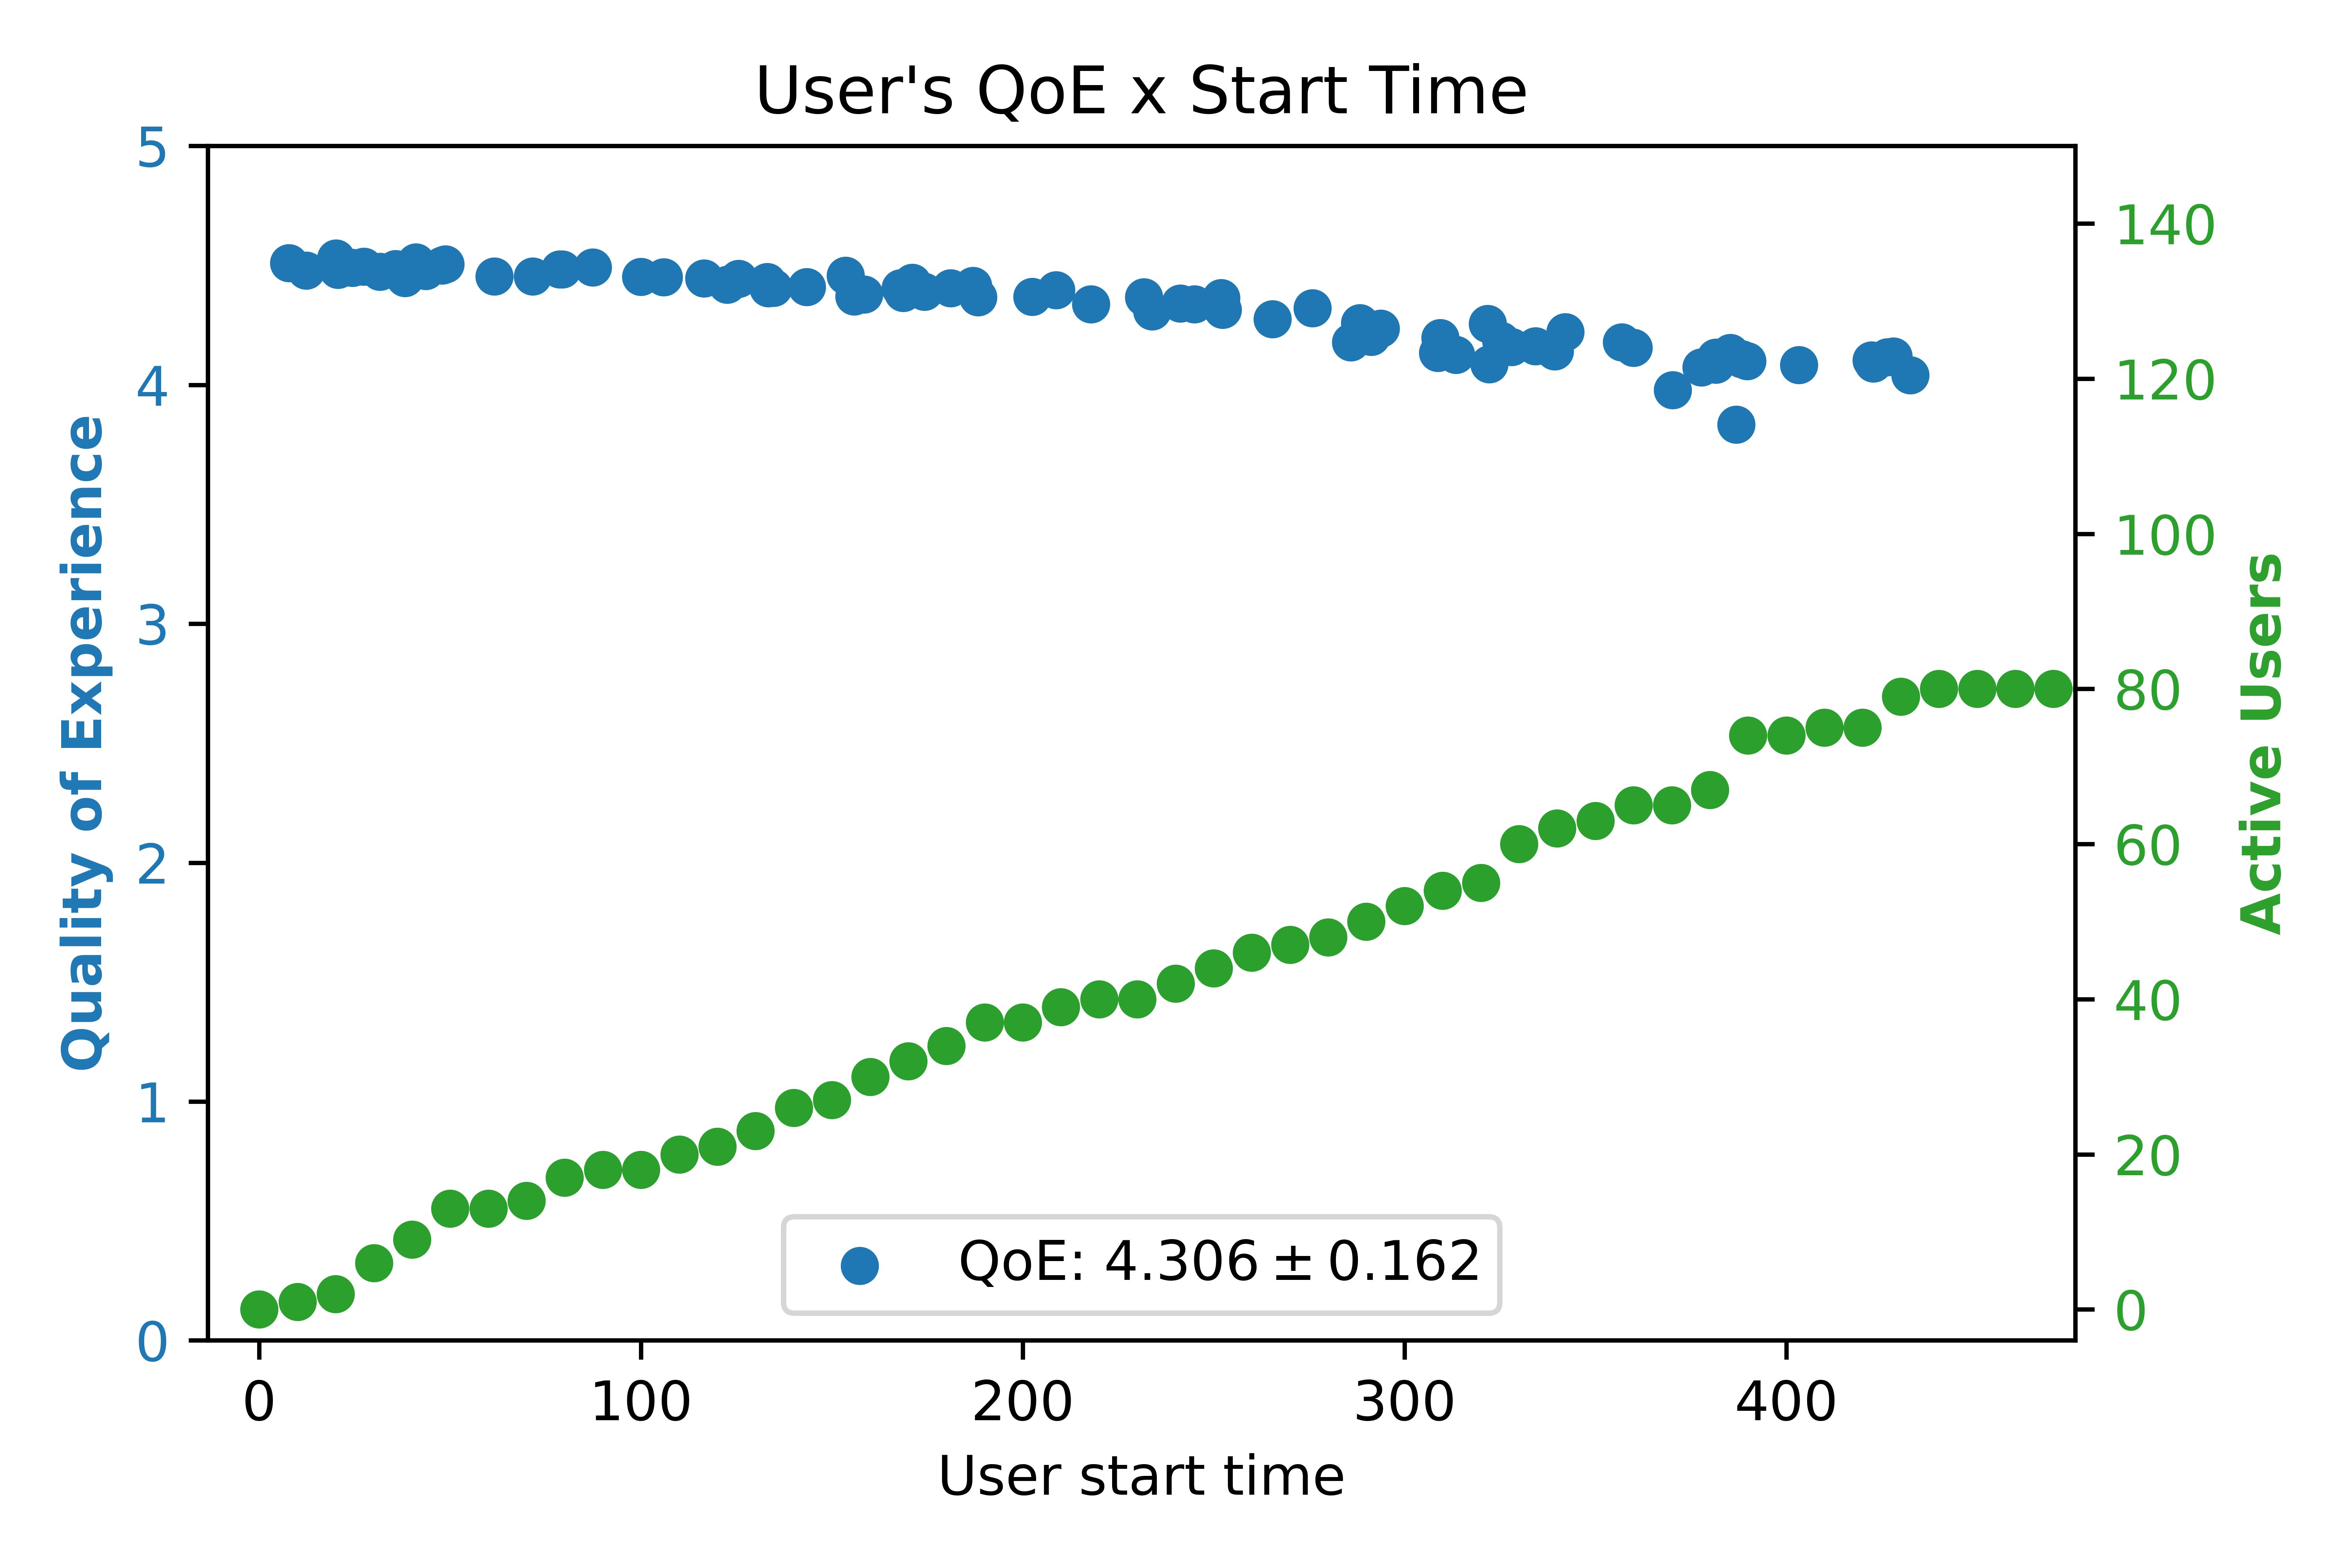
\includegraphics[width=0.31\linewidth]{images/Redicrect_QoExStartTime20.png}
    \label{fig:plr-comparison-2}
    }
    \subfigure[]{
    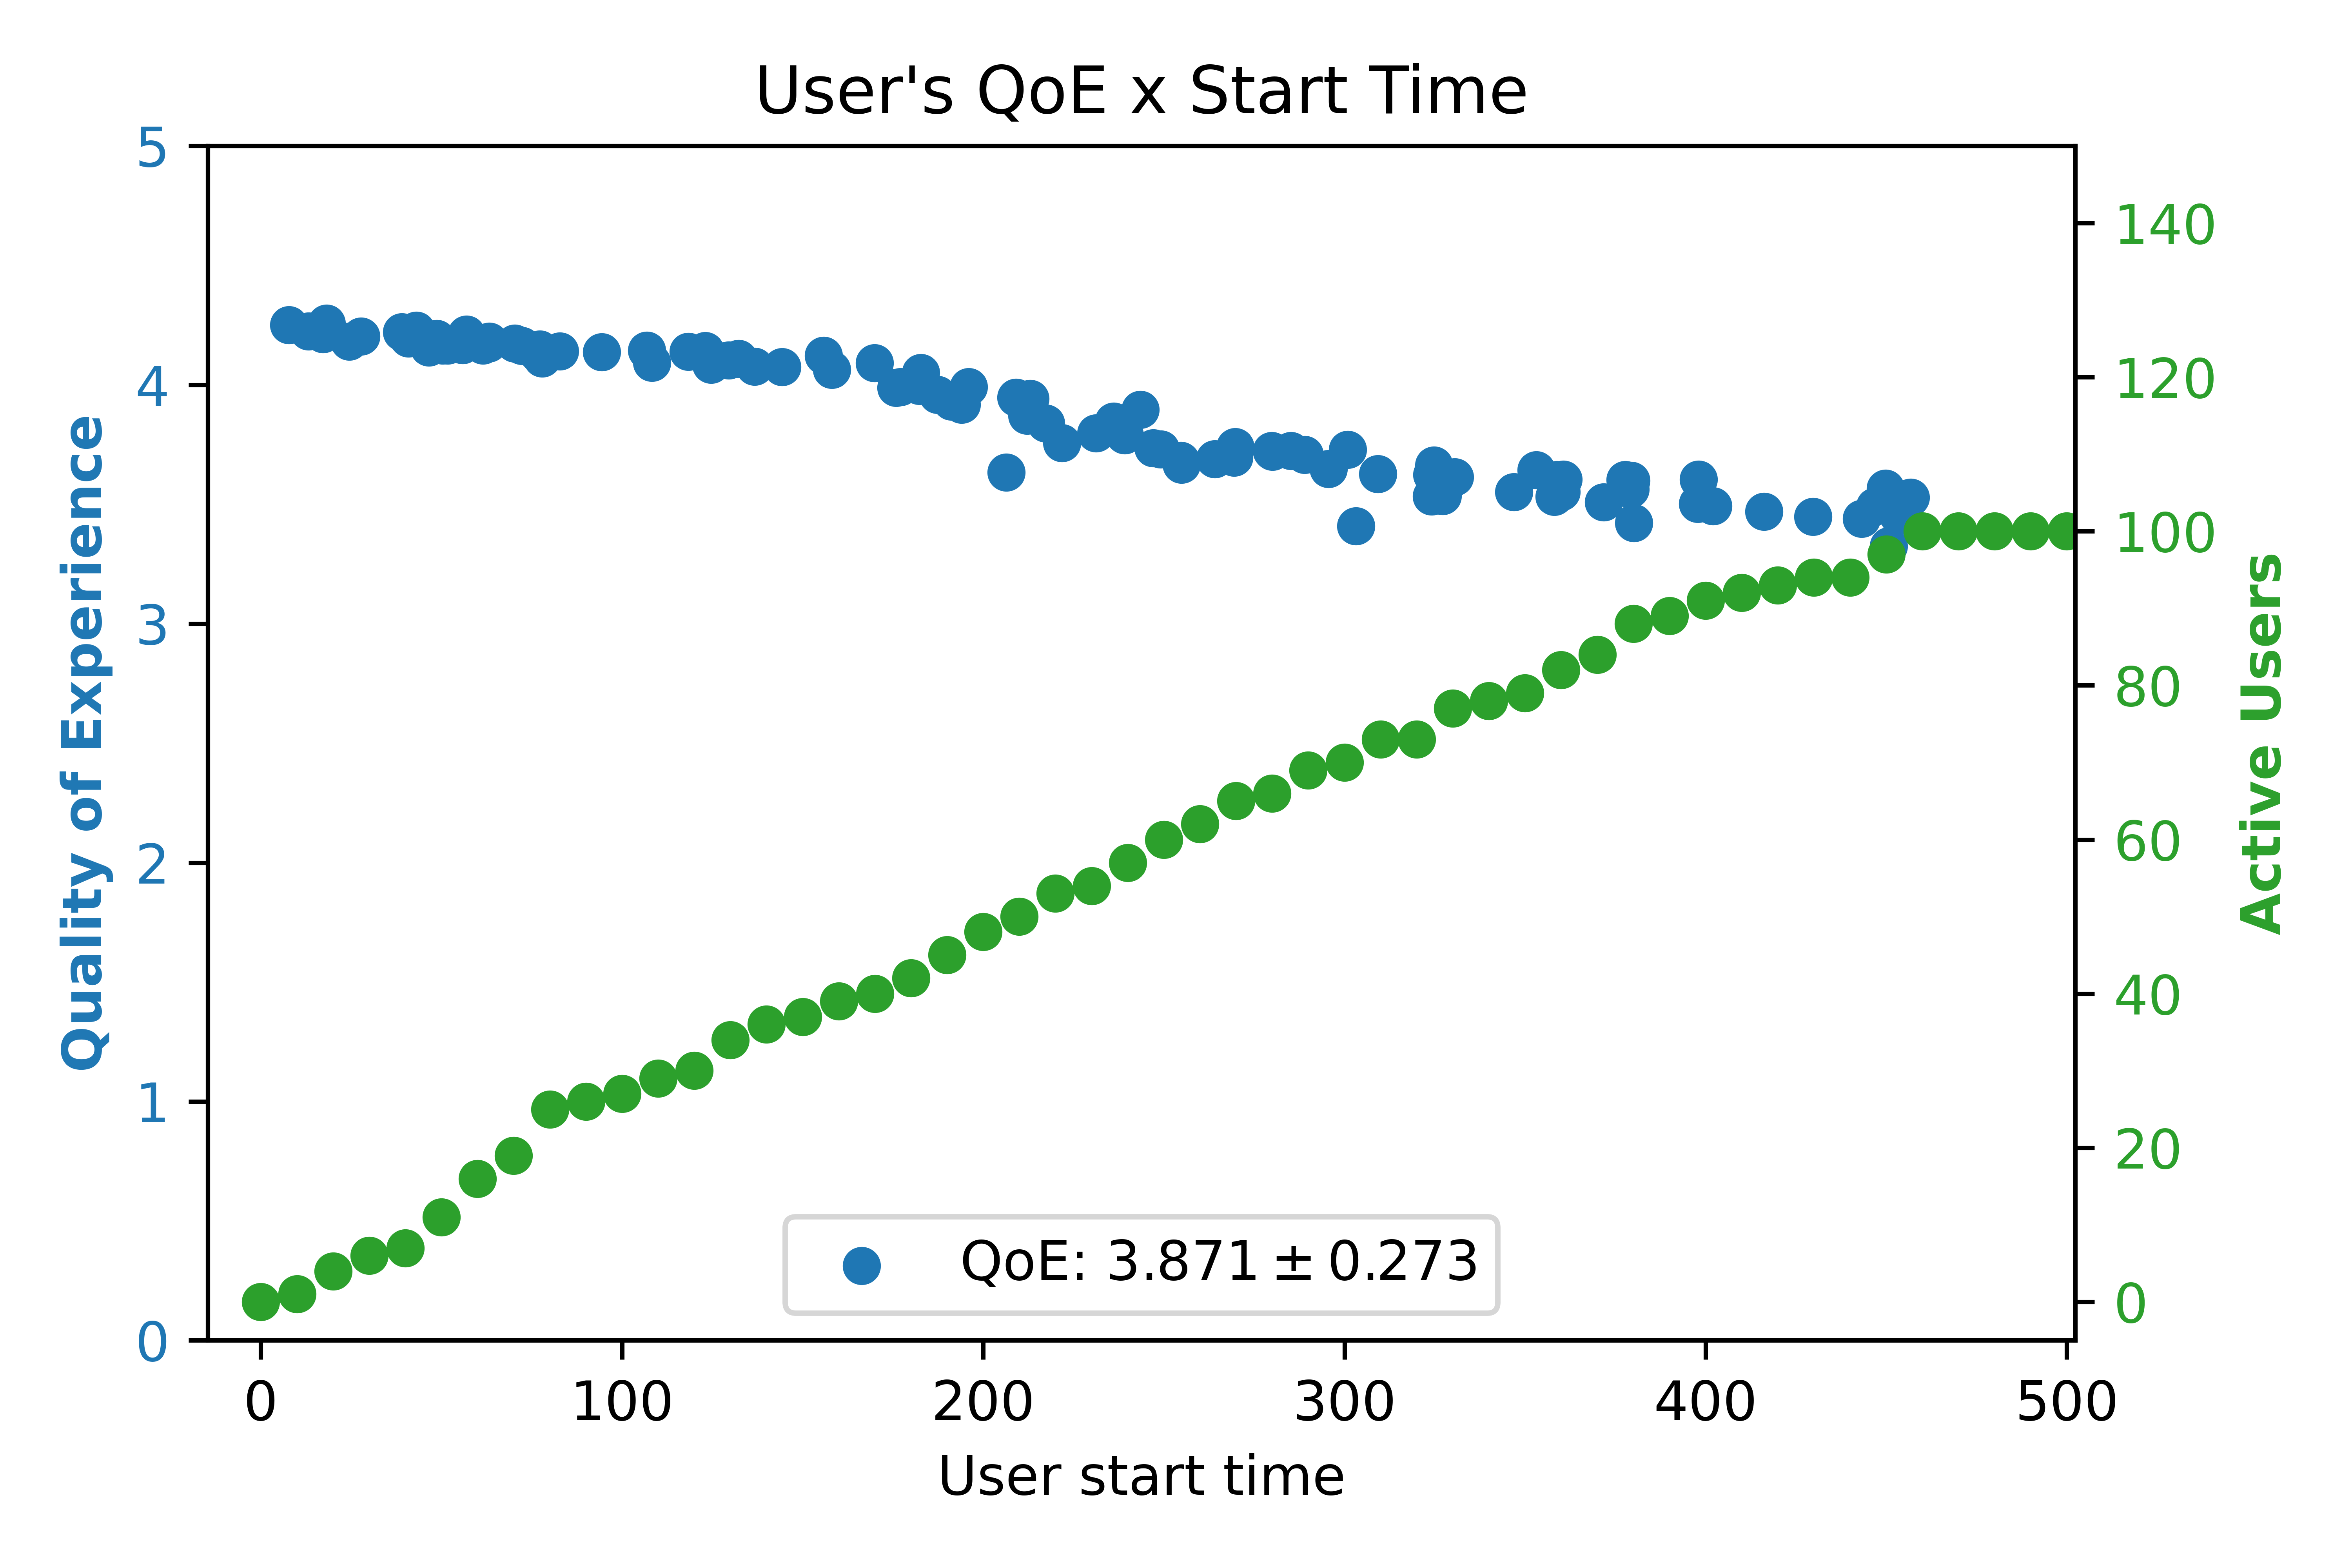
\includegraphics[width=0.31\linewidth]{images/Redicrect_QoExStartTime25.png}
    \label{fig:plr-comparison-2}
    }
    
    \caption{Impact of system on the network performance. Distance \textit{d} between sensor node and antennas of 8m in a semi-NLOS scenario.}
    \label{fig:comparison-qoe-2}
\end{figure*}

\subsection{Discussion and Results Summary}

%As mentioned earlier, the behavior of ABR schemes introduces the problem of selfish decisions when choosing the next segment to be requested. Obviously, different metrics of segment choices lead to different results in the status of buffer occupation and quality of the user's video, which results in a different QoE factor according to the heuristic used.

The experiments illustrated in Figures~\ref{fig:exp-boxplot-15}, \ref{fig:exp-boxplot-20} and \ref{fig:exp-boxplot-25} show the average QoE calculated by~Eq.~\ref{eq:qoe-equation} to 15, 20, and 25 users. Each boxplot represents the Cloud-only, 1\&2 node and mobility scenarios. As seen, the overall average performance of the 1\&2 is higher than the Cloud-only and mobility. Mainly due to the choices of nodes at the edge peering nodes for serving the requests done by users. 
%
For instance, for a 1\&2 experiment, when a congestion occurs in intermediate links $e_{0,1}$ e $e_{0,2}$, 
the edge peering nodes are activated to serve the end-users below those nodes. In this way, the traffic passing through the link above will now be smoothed out, so the users can improve their resulting QoE to an excellent level.
%edge peering nodes are activates para atender os usuários abaixo desses nós. Desta forma, os trafego que estava passando pelos link acima agora vão ser suavizados, assim os usuários conseguem melhorar seu QoE resultante para um nível excelente.    
%
Since the users request the segments by the closer nodes and with no congestion link in scenarios 1\&2, it is evident that as the QoE increases. %Remember that the scenario 1\&2, there is a link congestion monitoring, so when a congestion link is detected, the cache node above the link is activated, and the users are redirected to request the video from the cache node.
%
The performance difference of the Cloud-only and mobility is near one order of satisfaction for 15 and 20 users and approximately two~three orders of satisfaction with 25 users.


\begin{figure}[!h]
    \centering
    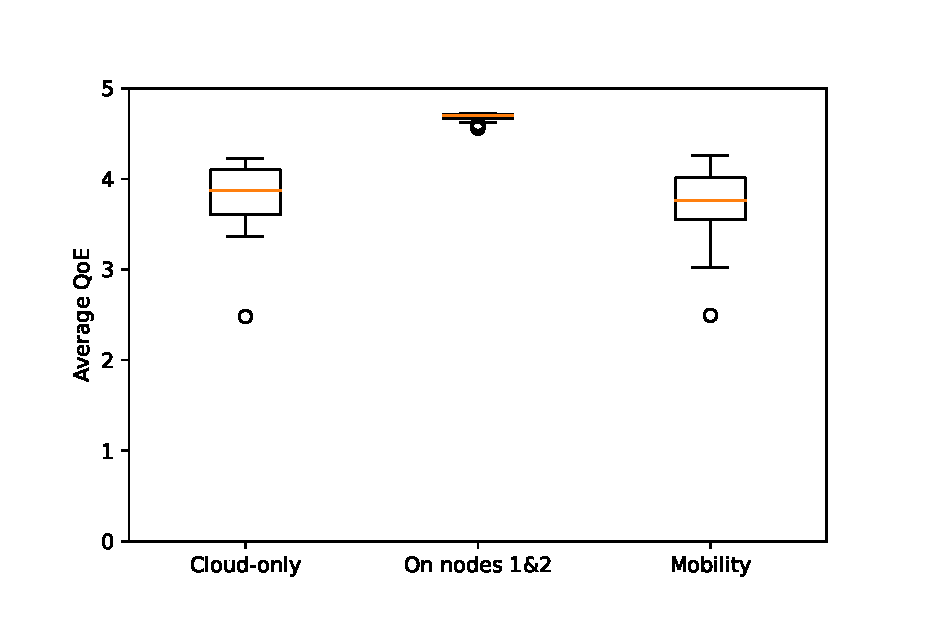
\includegraphics[width=\linewidth]{images/QoEBoxplot-15u.eps}
    \vspace{-0.9cm}
    \caption{Average QoE results for scenario with 15 users per AP.}
    \label{fig:exp-boxplot-15}
\end{figure}

\begin{figure}[!h]
    \centering
    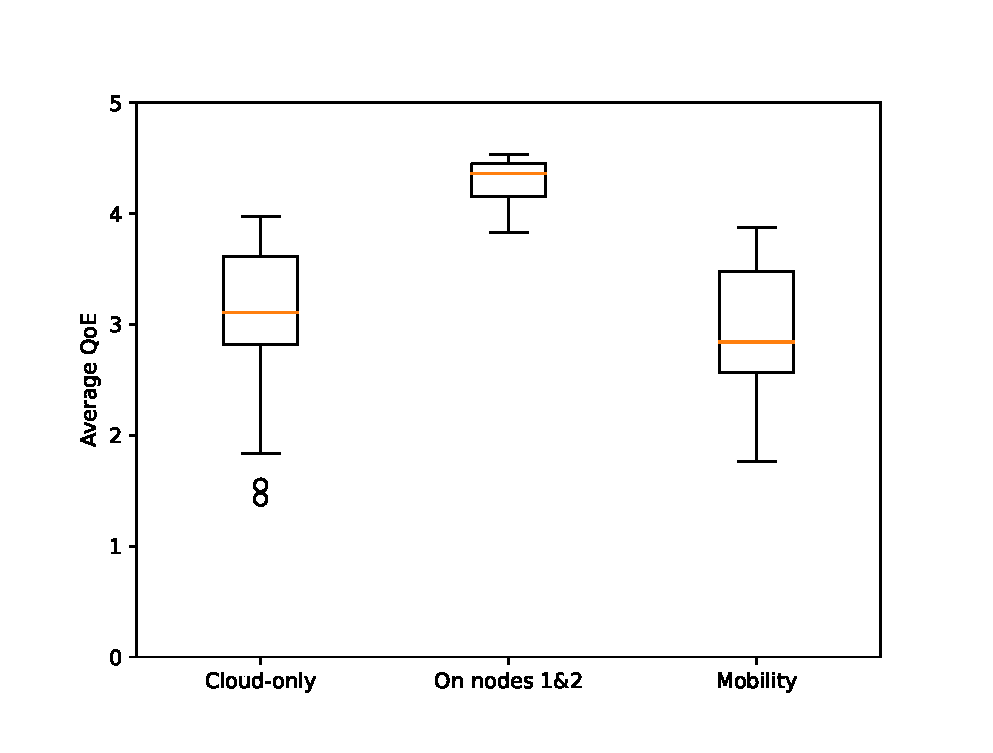
\includegraphics[width=\linewidth]{images/QoEBoxplot-20u.eps}
    \vspace{-0.9cm}
    \caption{Average QoE results for scenario with 20 users per AP.}
    \label{fig:exp-boxplot-20}
\end{figure}

\begin{figure}[!h]
    \centering
    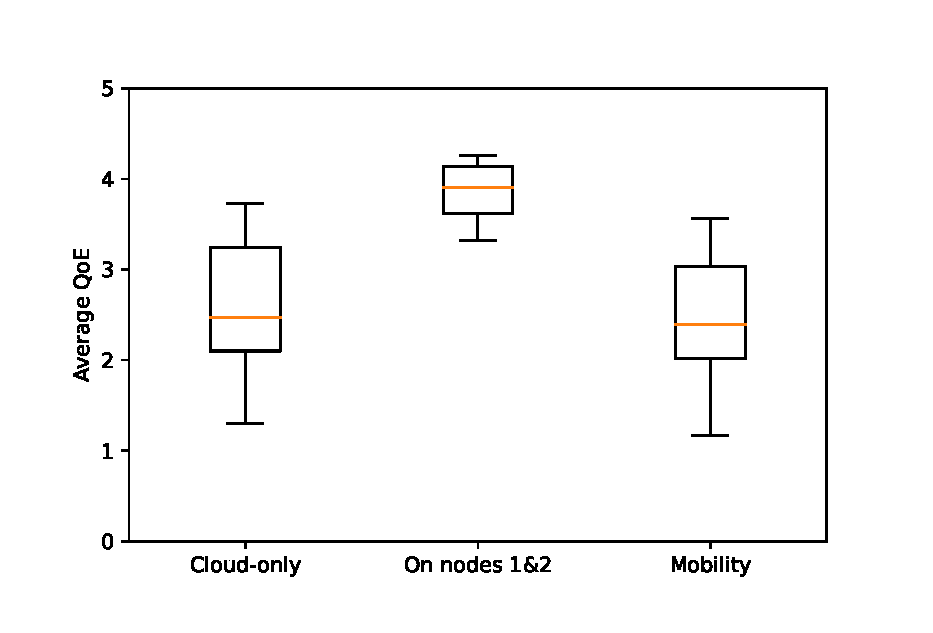
\includegraphics[width=\linewidth]{images/QoEBoxplot-25u.eps}
    \vspace{-0.9cm}
    \caption{Average QoE results for scenario with 25 users per AP.}
    \label{fig:exp-boxplot-25}
\end{figure}


It is important to note that the QoE results of scenarios after mobility are similar to the results of Cloud-only, even that the edge peering nodes using the QoE. This is due to the lack of a rerouting mechanism in real-time when users switch to another AP. The connections between the edge peering nodes and the users remain unchanged, so that the paths through which the packets pass are worse, negatively impacting the performance of the network as a whole.
%Another point to be noted is the average bit rate between different levels. In the scenario with 20 users, level 3 was able to achieve what is necessary to obtain the highest bit rate representation, thus, network operators can seek to deploy caches during peak hours to provide the best user experience.

Figures~\ref{fig:exp-setup-15}, \ref{fig:exp-setup-20} and \ref{fig:exp-setup-25} show the QoE final of each user per start time~(time to start the segment requests). Here, we can see the final QoE degradation to each user's entrance during the simulation execution. The green plot represents the number of active users simultaneously.  
As users reach the final QoE in this experiment, it tends to be slightly lower than the previous one. When looking at the final QoE delta between users $u_{i}$ and $u_{i + 1}$ seem to be irrelevant, but as we increase the delta, the QoE starts to become considerable different. Through the figures we can also affirm this behavior, as the number of users increases, the average QoE decreases, and the variation between users increases. Also, note that in the simulation with 25 users per system, the system already shows a degradation in the quality negatively perceived by the end-user.

\begin{figure}[!h]
    \centering
    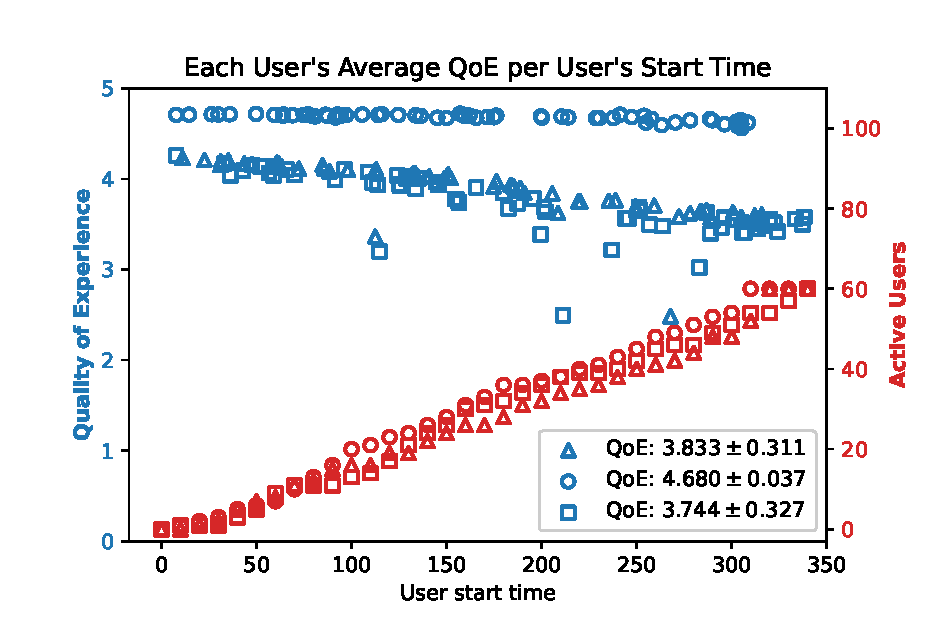
\includegraphics[width=\linewidth]{images/UserQoExUserStartTime15users.eps}
    \vspace{-0.7cm}
    \caption{Average QoE final results for each user with 15 users per AP.}
    \label{fig:exp-setup-15}
\end{figure}

\begin{figure}[!h]
    \centering
    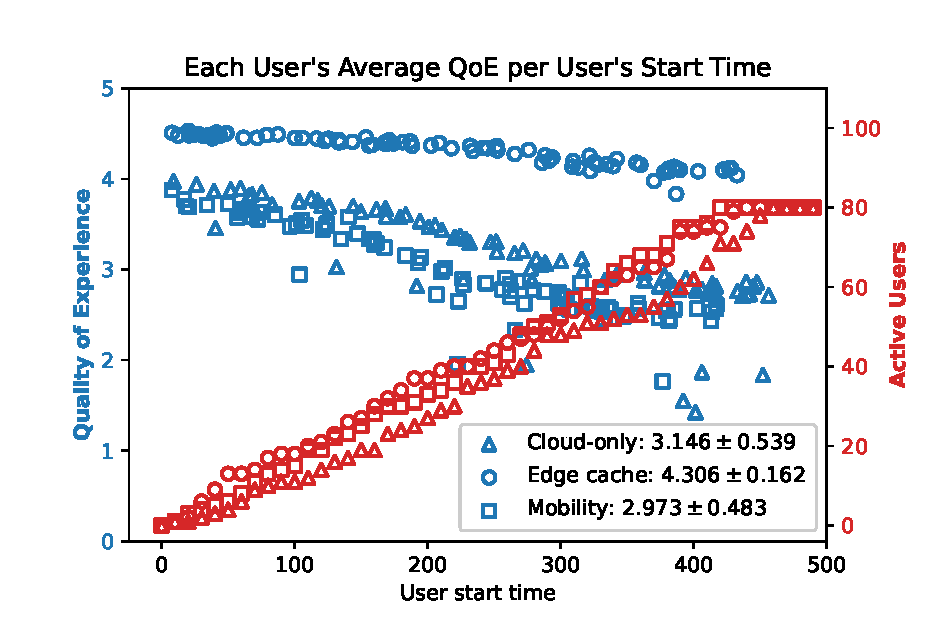
\includegraphics[width=\linewidth]{images/UserQoExUserStartTime20users.eps}
    \vspace{-0.7cm}
    \caption{Average QoE final results for each user with 20 users per AP.}
    \label{fig:exp-setup-20}
\end{figure}

\begin{figure}[!h]
    \centering
    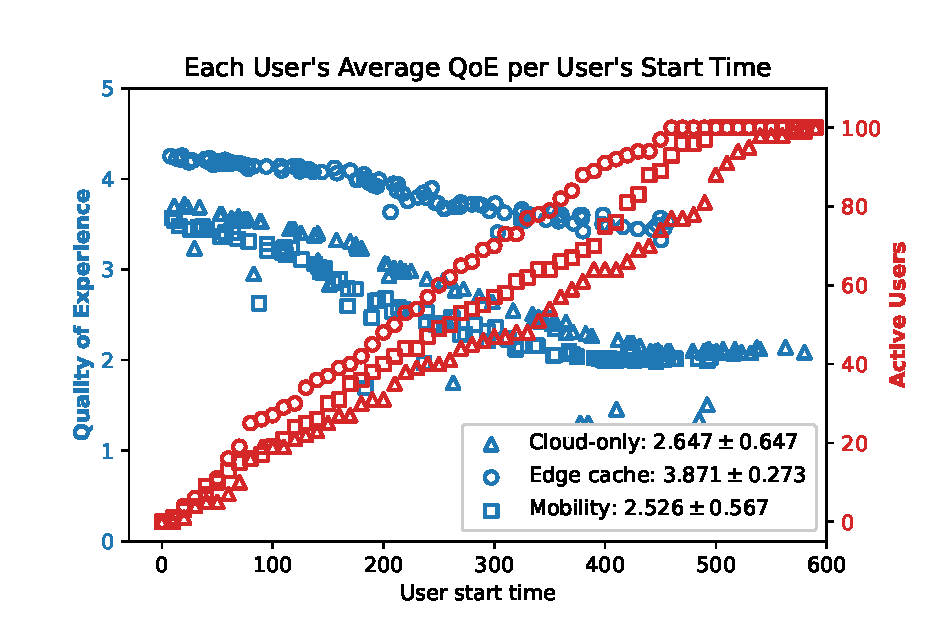
\includegraphics[width=\linewidth]{images/UserQoExUserStartTime25users.eps}
    \vspace{-0.7cm}
    \caption{Average QoE final results for each user with 25 users per AP.}
    \label{fig:exp-setup-25}
\end{figure}

Based on these observations,
a simple strategy of moving the video to the edge can significantly improve the user's QoE. In this way, the video transmission system can provide user satisfaction qualities and tend to keep them watching the video until the end.
However, if there is no correct management of connections in real-time, we can conclude that the impact introduced by the AP changes can significantly decrease the QoE for mobile users. The user experience can end up getting worse even using the edge of the network. Proper management of multimedia content can be done in which the VoD focus the decision-making in provide a a better QoE for the users changes. A simple content migration within the own edge in a upper tier can solve the problem, as well as realize a rerouting between the active users connections and the server nodes. 

%Based on these observations,
%a simple strategy of moving the video to the edge can significantly improve the user's QoE. In this way, the video transmission system is able to provide user satisfaction qualities as well as they tend to keep them watching the video until the end. 
%Contudo, caso não ocorra um correcto management das conexões em tempo real,  we can conclude that the impact introduced by the AP changes can decrease significantly the QoE for mobile users. A experiencia do usuário pode acabar se tornando pior mesmo usando a borda da rede. Um gerenciamento adequado do conteúdo multimidia pode ser feito de modo que uma simples migração do conteúdo dentro da borda pode solucionar o problema.

\section{Conclusion}
\label{sec:conclusion}

%Through a controlable scenario, it can be seen that there are many proposals in the area of ​​adaptive video streaming that do not take into account essential aspects of the user's QoE discussed in this work. In addition, current work on DASH architectures for future generations of smart grids ignores the behavior of the video player in Smart City environments. ,  On the client side, aspects of the way in which the video player behaves to provide a delicate balance between cost and customer satisfaction (in terms of QoE), as well as the impact that the insertion of cross traffic can have on the viewer . While on the server side, new simulation scenarios with different domains between nodes in the mist need to be considered, as well as performing the communication between these domains in multilevel environments.

The characteristics of a multi-tier edge/cloud scenarios with a VoD service was investigated. Numerical results for a binary tree network suggest that the correct video management result in a substantial improvement in the users' QoE. However, introduzindo uma simples troca de conexões entre os usuarios e Aps, a falta de um orchestramento adequado das conexões podem impactar negativamente a satisfação do usupario.

In the continuation of this work, we intend to implement mechanisms capable of orchestrating the users' connections in real-time and improving the provisioning of video streaming in multi-tier fog/cloud environments.
Another improvement is assessing how service behaves to provide a delicate balance between cost and customer satisfaction in terms of QoE.

%This work proposes a multi-tier architecture with a set of video-related services. The services were designed following the ETSI-NFV architecture. It focuses on the demonstration of the suitability of the services for multi-tier fog/cloud envi- ronments. In doing that, several properties of fog computing were further characterized. The proposed work combines recent fog/cloud technologies with state-of-the-art multi- tiered computing environments. This justifies the need for investigating specific services for video streaming provision- ing. As future work, we intend to implement the principles of NFV-SDN-based on


\section*{Acknowledgment}

This work was partially supported by the grant \# 2018/02204-6, São Paulo Research Foundation (FAPESP) and by the European Commission H2020, \# 688941 (FUTEBOL), as well from the Brazilian MCTIC through RNP and CTIC.

\begin{small}
    \bibliographystyle{unsrt}
    \bibliography{references}
\end{small}

\vspace{12pt}

\end{document}
